\documentclass[10pt,twocolumn,twoside]{article}
\usepackage[T1]{fontenc}
\usepackage[utf8]{inputenc}
\usepackage{amsfonts, amsmath}
\usepackage[backend=biber, style=numeric-comp, citestyle=nature, doi=false, isbn=false, url=false, eprint=false]{biblatex}
\addbibresource{cimodel.bib}
\usepackage[margin=0.85in]{geometry}
\usepackage{fontspec}
\setmainfont{Carlito}
\usepackage{hyperref}
\hypersetup{
	colorlinks = true, %Colours links instead of ugly boxes
	urlcolor = blue, %Colour for external hyperlinks
	linkcolor = red, %Colour of internal links
	citecolor = red %Colour of citations
}
\usepackage{threeparttable}
\usepackage{graphicx}
\usepackage{fancyhdr}
\pagestyle{fancy}
\fancyhf{}
\rhead{\thepage}
\makeindex

\usepackage{authblk}
\author[1]{Vibishan B.}
\author[1,*]{Milind G. Watve}
\affil[1]{Department of Biology, Indian Institute of Science Education and Research (IISER), Pune}
\affil[*]{Corresponding author: milind@iiserpune.ac.in}

\title{Context-dependent selection as the keystone in the somatic evolution of cancer}

\begin{document}

\maketitle

\section{Introduction}

Mathematical models of somatic evolution in cancer have been in development for the past several decades, with a strong focus on mutational processes \cite{ARMITAGE1954, McFarland2013, Blokzijl2016, Mina2017}. Most prominently, Tomasetti et al. have argued that cancer risk is largely determined by random mutations \cite{Tomasetti78, Tomasetti2017}. On the other hand, the question of somatic evolution in cancer parallels an old debate in the theory of evolution as to how the simple process of random mutations alone can lead to complex structures such as the eye which require the coordinated action of several genes, often perceived as the monkey-on-a-typewriter paradox \cite{Dawkins1996}. The problem of cancer is qualitatively similar to this, but quantitatively even more difficult, since most cancers must evolve independently in each individual organism. All cancers are necessarily a combination of different types of genomic changes including point mutations, aneuploidy and other chromosomal aberrations, and the cancer phenotype has a large number of distinguishing characeters, encapsulated by the notion of the ``hallmarks'' of cancer \cite{Hanahan2000, Schafer2008, Hanahan2011}. The wide range of characterisitics that these hallmarks include make it astonishing that so many alterations in cell properties come together in cancers purely out of chance.

Selection on intermediate mutants was the logical solution provided for the monkey-on-a-typewriter paradox, and clonal expansion paralleled such a solution in cancer evolution. Every component mutation on the way to a cancerous phenotype causes the mutant clone to expand, and as the mutant population increases, the probability of a second component mutation increases proportionately \cite{Nowell1976}. Implicit in this theory is the assumption that every component mutation has a selective advantage over the normal cell. Since most changes involved in carcinogenesis relate to evading growth regulatory mechanisms, it is considered logical that any mutation that allows for such evasion will have a natural selective advantage. However, evidence has been accumulating over the past few years that the fitness advantage of a mutant is largely dependent on the tissue micro-environment \cite{Hanahan2012, Pietras2010}. Studies in mice \cite{Cao2010} and humans \cite{Rundqvist2013} have demonstrated the effect of contingent factors, such as behavioural profiles and lifestyle parameters, on cancer progression. These findings provide clear indications that the selective forces which determine mutant clone fitness can vary considerably across individuals, leading to \textit{context-dependent clonal expansion} of potentially oncogenic mutants. The role of such differential selective forces in somatic evolution has not been adequately addressed by cancer models so far.

In this paper, we compare three modelling approaches, two of which explicitly include selection at different levels: (1) random mutagenesis, or the ``bad luck'' hypothesis, (2) context-independent expansion of mutant clones within individuals, and (3) context-dependent selection acting across individuals. Since well-curated data are available for human cancer incidence patterns through the SEER databases \cite{AmericanCancerSociety2016}, we develop models of these three processes, and compare their predictions with the epidemiological picture of cancer in the human population.

A good working model of somatic evolution of cancer needs to explain the following epidemiological features:

\begin{enumerate}
	\item Total and age-specific incidence: Total incidence of cancer across types lies below 30\%, while age-specific and cumulative incidence patterns show more variations between cancer types \cite{AmericanCancerSociety2016}. Interestingly, recent analyses have shown for several cancers that the age-specific incidence rates decline late in life \cite{Harding2012}, in contrast with general model predictions of a power law increase in incidence with age (some theoretical explanations for this decline have been suggested \cite{Frank2007}). The late-life decline causes the cumulative incidence to saturate with age at a small percentage of the population size. No matter the lifespan, the proportion of cancer in the population can never reach 100\%, which represents a finite limit that is not determined by time.
	\item Incidence vs cell number: As mentioned earlier, the relationship between cancer risk and cell number (as the lifetime number of cell divisions, \textit{lscd}) has been kept in the spotlight by recent work by Tomasetti et al. \cite{Tomasetti78, Tomasetti2017}. Although the linearity of the relationship between \textit{lscd} and cancer risk is still under debate, available data can be used to comparatively test model predictions.
	\item Incidence vs mutation rate: Empirical data on this relationship are less common, as mutation rates are difficult to measure reliably, although some efforts have been made \cite{Hao2016}. However, a general notion exists that higher mutation rates increases cancer risk, and this remains to be tested rigorously, barring theoretical work dealing with the effect of mutagens on patterns in incidence data \cite{Frank2007}.
	\item Non-mutagenic carcinogens: There are several agents, including hormones and growth factors, that increase cancer risk without affecting the basal mutation rate \cite{Tennant1993}. The activity of these agents, and their signature in epidemiological patterns, are both important in building a complete framework of explaining cancer etiology.
	\item Peto's paradox, and similar observations: This relates to the incidence-cell number relationship, as cancer risk is seen not to scale with body size or cell number across species \cite{Nagy2007}, with does correlate with the latter within a species \cite{Noble2015}. A wide range of explanations have been offered for this observation \cite{Tollis2017b}, and in a modeling context, these explanations can come from the model itself (intrinsic), or involve extrinsic factors, such as evolved cancer defences, that are not part of the model framework.
	%\item Mutational meltdown: While well-known in other study systems, the effects of deleterious mutations were recognized relatively recently in cancer literature.
\end{enumerate}


\section{The ``bad luck'' model}

This hypothesis assumes that the required set of driver mutations accumulate in a cell by chance alone. This may happen over a period of time, or in a single large-scale event, like chromothripsis \cite{Stephens2011}. Regardless of whether mutations accumulate sequentially or otherwise, the ``bad luck'' model does not assume selection of any kind on mutations over the course of somatic evolution.

Consider an organism with a population of $n$ stem cells, each with a mutation rate per cell generation per locus, $p$. The probability that at least one cell acquires one mutation at a given point of time can be given as $1-(1-p)^{n}$. If $k$ such mutations are requried for cancer onset, the probability of cancer according to the bad luck model can be given as below, based on an algebraic formulation \cite{Calabrese2010}:

\begin{equation}
	\label{E1}
	p_{can} = 1-(1-p^{k})^{n}
\end{equation}

Given the probability of cancer per unit time, $p_{can}$ from equation \ref{E1}, the cumulative incidence of cancer for age, $A$, can be expressed as below:
\begin{equation}
	\label{E2}
	p_{A} = 1-(1-p_{can})^{A}
\end{equation}

From equation \ref{E1}, it is clear that the probability of cancer has a threshold relationship with both $n$ and $p$, such that incidence rises from near zero to 100\% over a small range of $p$ and $n$, as shown in Figure \ref{fig1}. Within this narrow range, total incidence as reflected by the cumulative probability, $p_{can}$, occasionally lies in the realistic range of about 30\%, but these are the exceptions.

\begin{figure*}[tbhp]
	\centering
	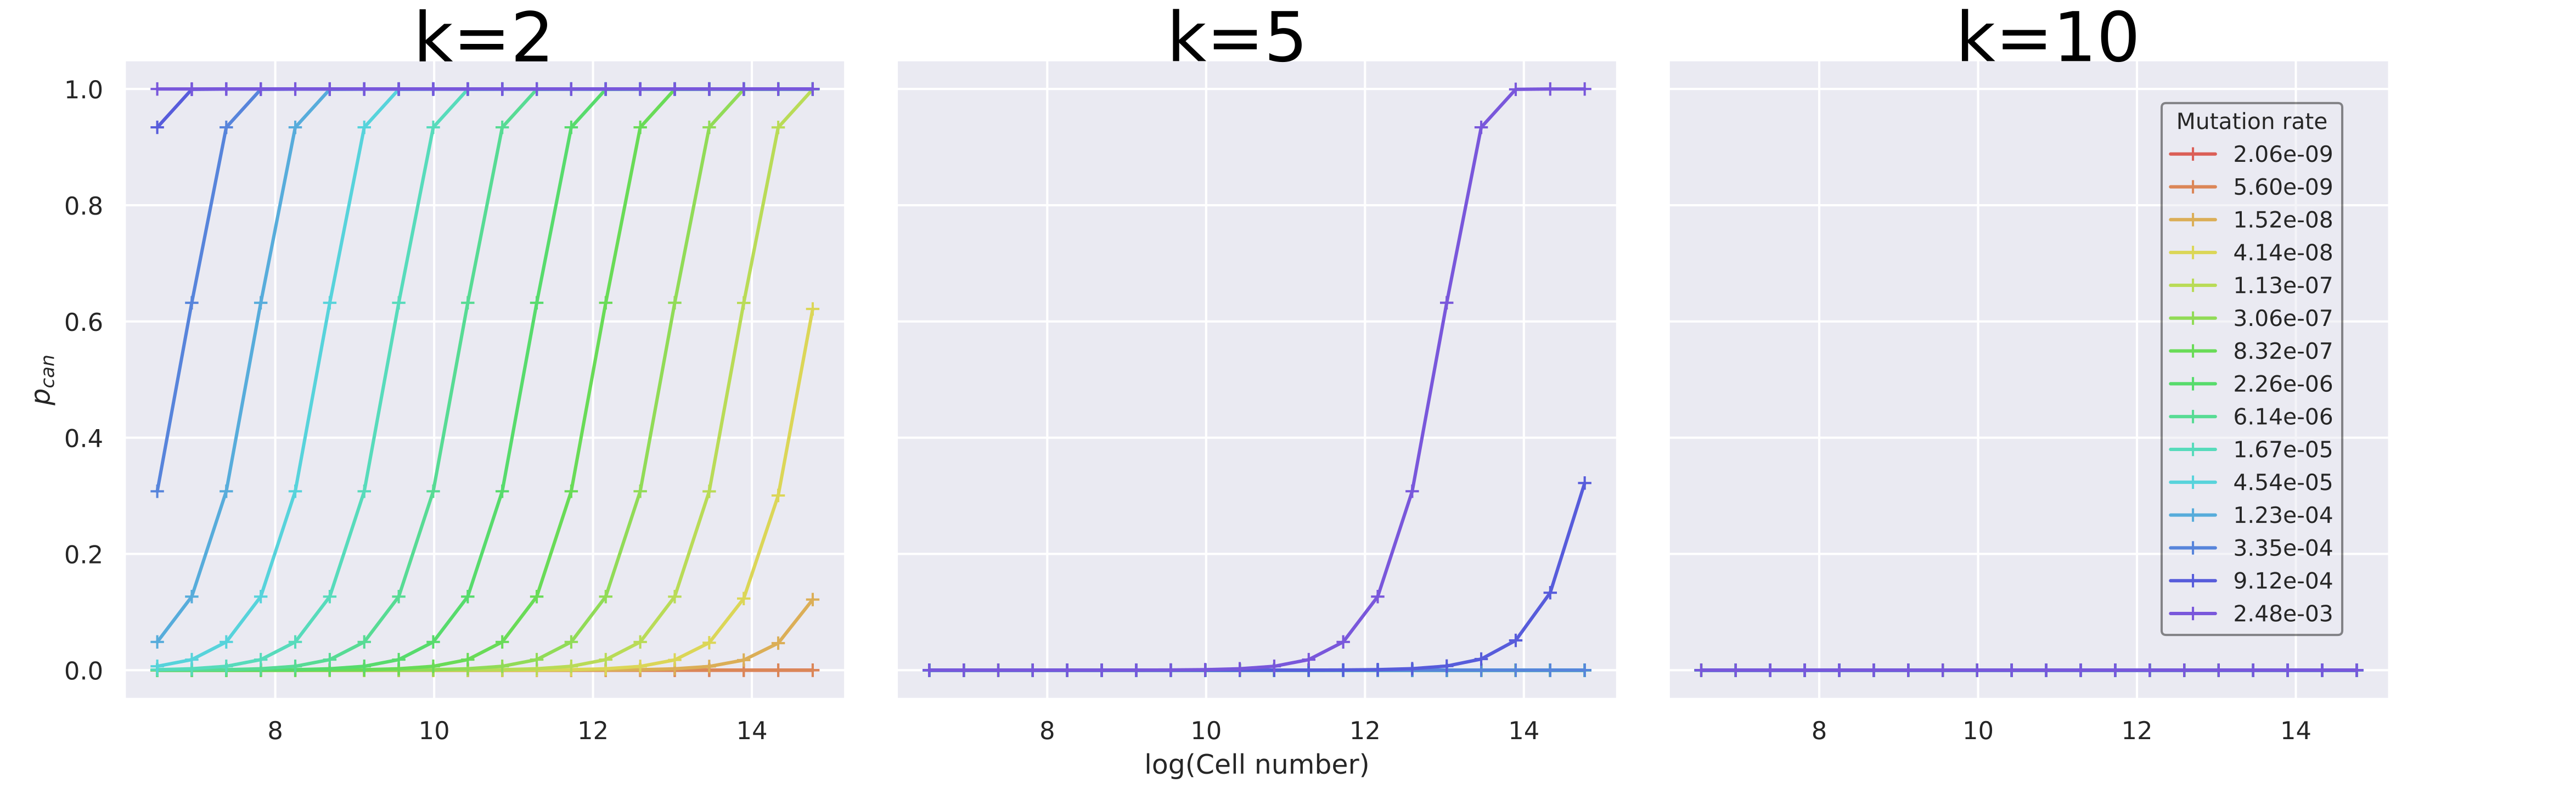
\includegraphics[width=\linewidth]{fig1.png}
	\caption{Cancer probability, $p_{can}$ vs cell number for the ``bad luck'' model; $p_{can}$ remains near zero in part of the parameter range, and rises to one over a narrow region of the corresponding parameter. This proability is cumulative and therefore reflects total incidence in the population. For the ``bad luck'' model, the total incidence is rarely in the observed range of around 30\%. The number of oncogenic mutations required for cancer onset ($k$) does not affect the existence of a threshold with $n$ and $p$, but does affect where the threshold occurs in the parameter space; for $k=10$, the threshold does not occur within the tested range of $n$ and $p$. The legend shows values of $p$ for each curve.}
	\label{fig1}
\end{figure*}

From equation \ref{E2}, the relationship of $p_{can}$ with age is a monotonically increasing function with a maximum at one. Figure \ref{fig2} shows this relationship across the entire parameter range of $n$ and $p$, for which this prediction holds. Cancer probability increases monotonically with age, and only saturates at 100\% incidence, which stands in stark contrast to the observed late-life decline in age-specific rates. Given a finite lifespan, cancer incidence lies in a realistic range in a narrow range of $p$ and $n$.

\begin{figure}[tbhp]
	\centering
	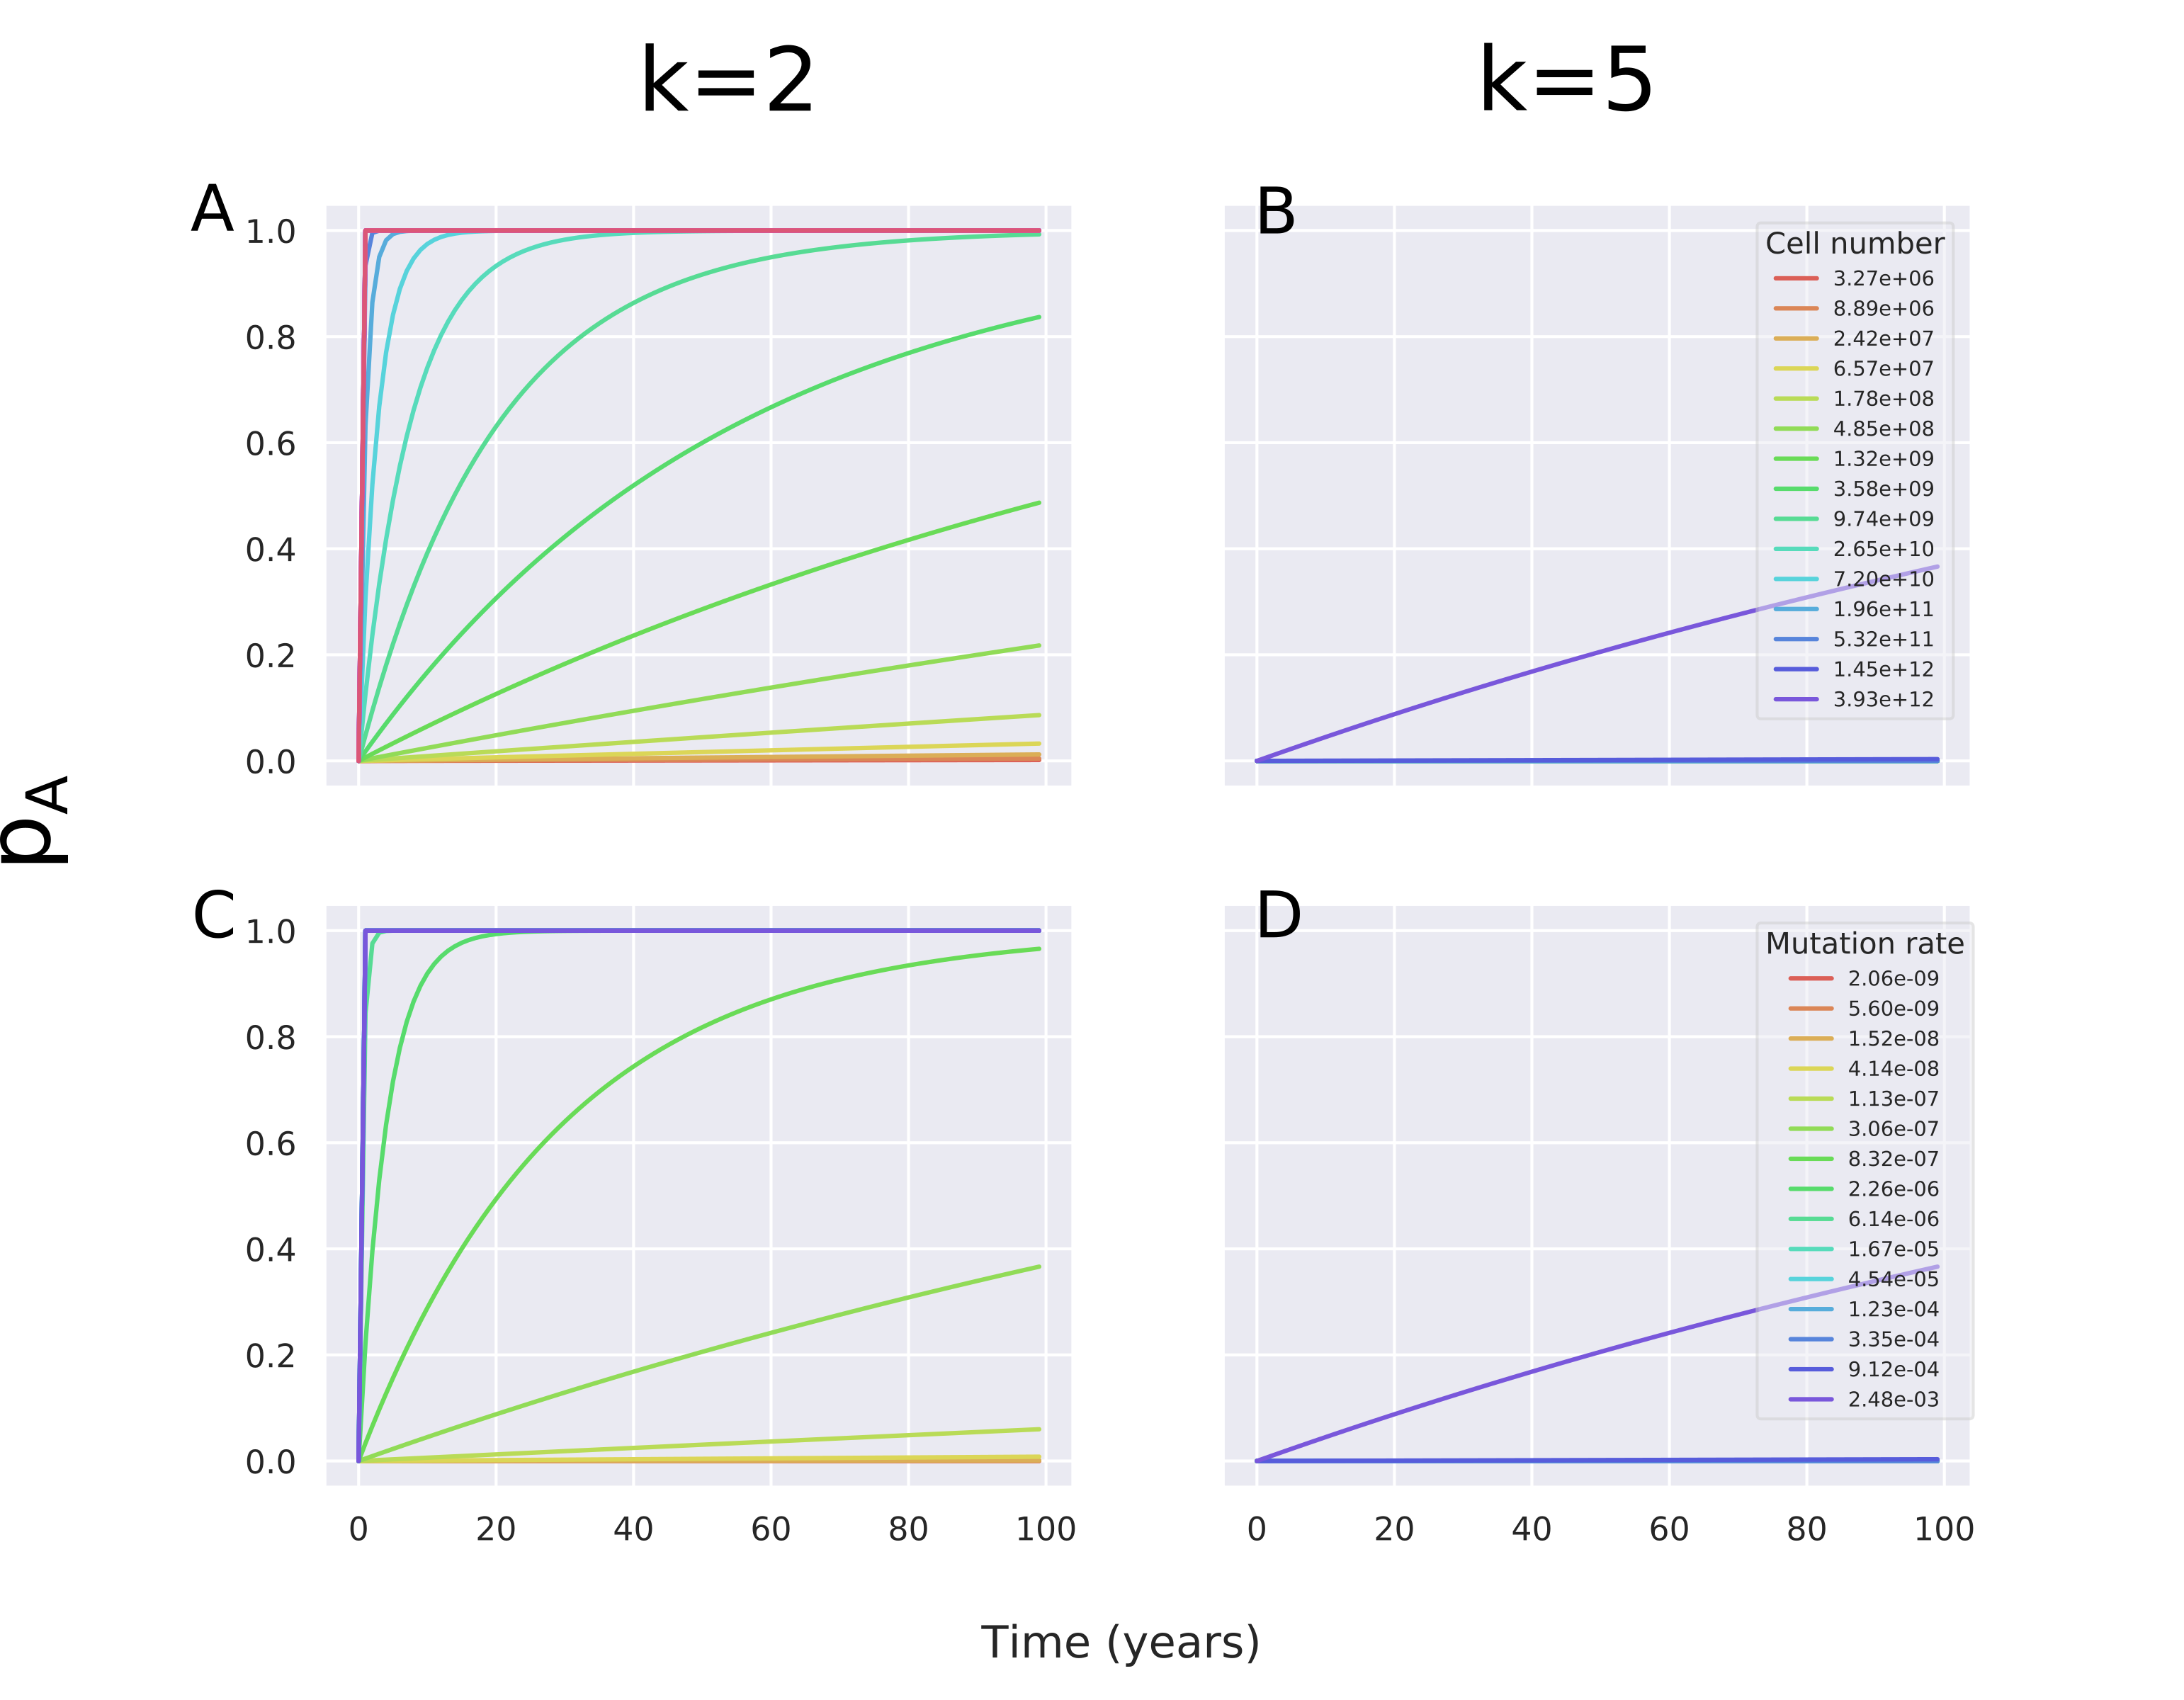
\includegraphics[width=\linewidth]{fig2.png}
	\caption{Cancer probability vs age, as given by equation \ref{E2}, (A and B) over the range of $n$, and (C and D) over the range of $p$; inset legends give the corresponding values of $n$ and $p$. Cancer probability increases monotonically with age, saturating only at one in most cases. Where the probability does approach realistic values of total incidence, it still does not reflect the late-life decline in incidence rates observed epidemiologically. As in Figure \ref{fig1}, the number of oncogenic mutations required for cancer onset does not change the nature of the incidence-age relationship. For A and C, $k=2$, and for B and D, $k=5$.}
	\label{fig2}
\end{figure}

Including the cost of lethal/deleterious passenger mutations does not qualitatively alter the general prediction of thresholds with $n$, $p$ and age, although the position of the threshold may change, as has been observed independently \cite{McFarland2013}. Taken together, this formulation of the ``bad luck'' model predicts a sharp threshold relationship of cancer probability with both $n$ and $p$, as opposed to the observed progressive increase \cite{Tomasetti78, Tomasetti2017}. For values of $n$ and $p$ around this threshold, cancer probability increases progressively with age but is inconsistent with late-life decline in cancer incidence. 
%We also used values of $n$ and $p$ for about 15 cancer types, along with the corresponding lifetime incidence of cancer from published literature \cite{Tomasetti78, Hao2016}, to carry out a chi-square test to compare the predictions of the ``bad luck'' model with the SEER incidence. A quick calculation is sufficient to show that the former predicts 100\% incidence for all tested cancer types, which is clearly unrealistic.

\section{Models with selection on mutants}
For models that involve selection, we choose to explore the effects of context-independent clonal expansion and context-dependent selection through a simulation-based stochastic framework. 

We use a linear process to model the sequential accumulation of mutations in a population of stem cells. We begin by considering the development of a generalized tissue compartment in each organism starting from one stem cell, with mutation rate per cell generation per locus, $p$, growing logistically to a carrying capacity, $n$, following the discrete logistic equation below:
\begin{equation}
	m_{i, t} = m_{i, t-1} + m_{i, t-1}*g_{i}*(\dfrac{n-\sum_{i=0}^{k} m_{i, t-1}}{n}) - m_{i, t-1}*d
	\label{E3}	
\end{equation}

Here, $m_{i, t}$ is the size of the $i$th mutant population at time, $t$, with $i=0$ being the non-mutant cell population, $g_{i}$ is the corresponding logistic growth rate, $d$ is the common death rate, and $k$ is the threshold number of oncogenic mutations required for cancer onset. As the organism develops into an adult, net growth in the stem cell compartment saturates, but reaches a dynamic equilibrium between cell death and renewal. The stem cell population can be reduced, either by death of stem cells or differentiation, as reflected by the death rate in equation \ref{E3}. Assuming a common death rate for all cell populations, the replacement of the lost cells by either mutants or non-mutants is a function of their growth rates. We simulate new mutation events stochastically; the probability of at least one cell accumulating a mutation is given by $1-(1-p)^{m_{i, t}}$, and if this probability exceeds a random number between 0 and 1, a new $(i+1)$th cell population is initiated. Each new oncogenic mutation could give a growth advantage over older cell populations, leading to successive cycles of clonal expansion in which the newer population gradually replaces older cells through competitive exclusion. We simulate this linear evolution process until $k$ mutations have been accumulated, which is the assumed threshold for cancer onset. Death of the individual occurs either at cancer onset when the $k$th mutation occurs, or at the end of the natural lifespan of 100 years, whichever happens first. This simulation is repeated independently for a population of 10000 individuals, and the population-level cancer incidence is recorded, along with the age of onset.
	\subsection{Choice of parameter range}
	In order to standardize the discrete logistic simulation, we assume the time unit to be one day per logistic growth step. Most human organs complete development and maturation wihtin the first 10-20 years of the lifespan, and the final carrying capacity achieved is the adult stem cell number, ranging between $10^{6}$ and $10^{11}$ across different tissues (supplementary material from \cite{Tomasetti78}). Given the final population size and the time taken to reach it, a simple calculation based on the logistic equation shows the required growth rate for a non-mutant stem cell to be in the range of $0.00383$-$0.0131$. Starting from the non-mutant growth rate, $g_{0}$, growth rates are assumed to increase linearly for each subsequent mutant population. Ranges of $n$ and $p$ are retained as in the ``bad luck'' model.

	\subsection{The context-independent selection case}
	While the clonal expansion theory introduced the notion of selective advantages to oncogenic mutants, it makes the implicit assumption that identical mutations have the same selective advantage in every individual in which they occur; stated otherwise, individuals do not differ in their propensity for mutant clonal expansion. To capture this in the context-independent selection case, we use the same linear progression of growth rates for all individuals in the simulation.

	\subsection{The context-dependent selection case}
	As argued earlier, it is becoming increasingly clear that the competitive outcomes of identical mutations can depend strongly on the micro-environmental context in which cell competition occurs. In order for selection on mutants to be context-dependent in our model, we randomize the progression of growth rates during mutation accumulation. Each individual begins with the same $g_{0}$, but the progression of growth rates is randomized across individuals, such that individuals with large $g_{i}$ would progress faster towards cancer onset, while those with small, or negative values of $g{i}$ would never progress to a cancerous state as the mutant gets selected against. This produces variation across organisms for cancer propensity.
	%While we study a simple case by randomizing $\mu$, in principle, it should be possible to vary $g_{k}$ with respect any non-random context-dependent variable derived from real data sources. But as we show later, our simple case several interesting results by itself.

\subsection{Predictions from the selection models}
As in Figure \ref{fig3}, under the assumption of context-independent selection, the incidence of cancer shows a strong threshold relatioship with age, where up to a certain age, cancer is unlikely or rare, but increases rapidly to 100\% within a relatively short span of time. This is indicated by the fact that the cumulative incidence reaches 100\% within the individual lifespan, and the age-specific incidence falls to zero. As with the ``bad luck'' model, incidence has a threshold relationship wtih both $n$ and $p$, as reflected in the maximum cumulative incidence, $I_{max}$ (Figure \ref{fig3}D and H). The age at half-maximum incidence is a decreasing function of both $n$ and $p$ (Figure \ref{fig3}C and G). Moreover, saturation of incidence occurs only at 100\%, which is identical to the ``bad luck'' model, despite the inherently stochastic implementation of mutation occurrence. Where the incidence of cancer is near the realistic range, for small values of $p$ and $n$, the late-life decrease in incidence is still not reflected in the context-independent selection case. The prediction of 100\% incidence is due to the fact that all organisms in the population share the same growth rate progression for mutants. No other parameter in the model inherently precludes the accumulation of all $k$ oncogenic mutations in some individuals; giving a distribution to $p$ reduces the sharpness of the incidence threshold with age, but saturation of incidence remains at 100\% (Figure \ref{fig4}). 
%and the dynamics of accumulation is entirely a function of $p$ and $n$, along with stochastic variation.

\begin{figure*}[tbhp]
	\centering
	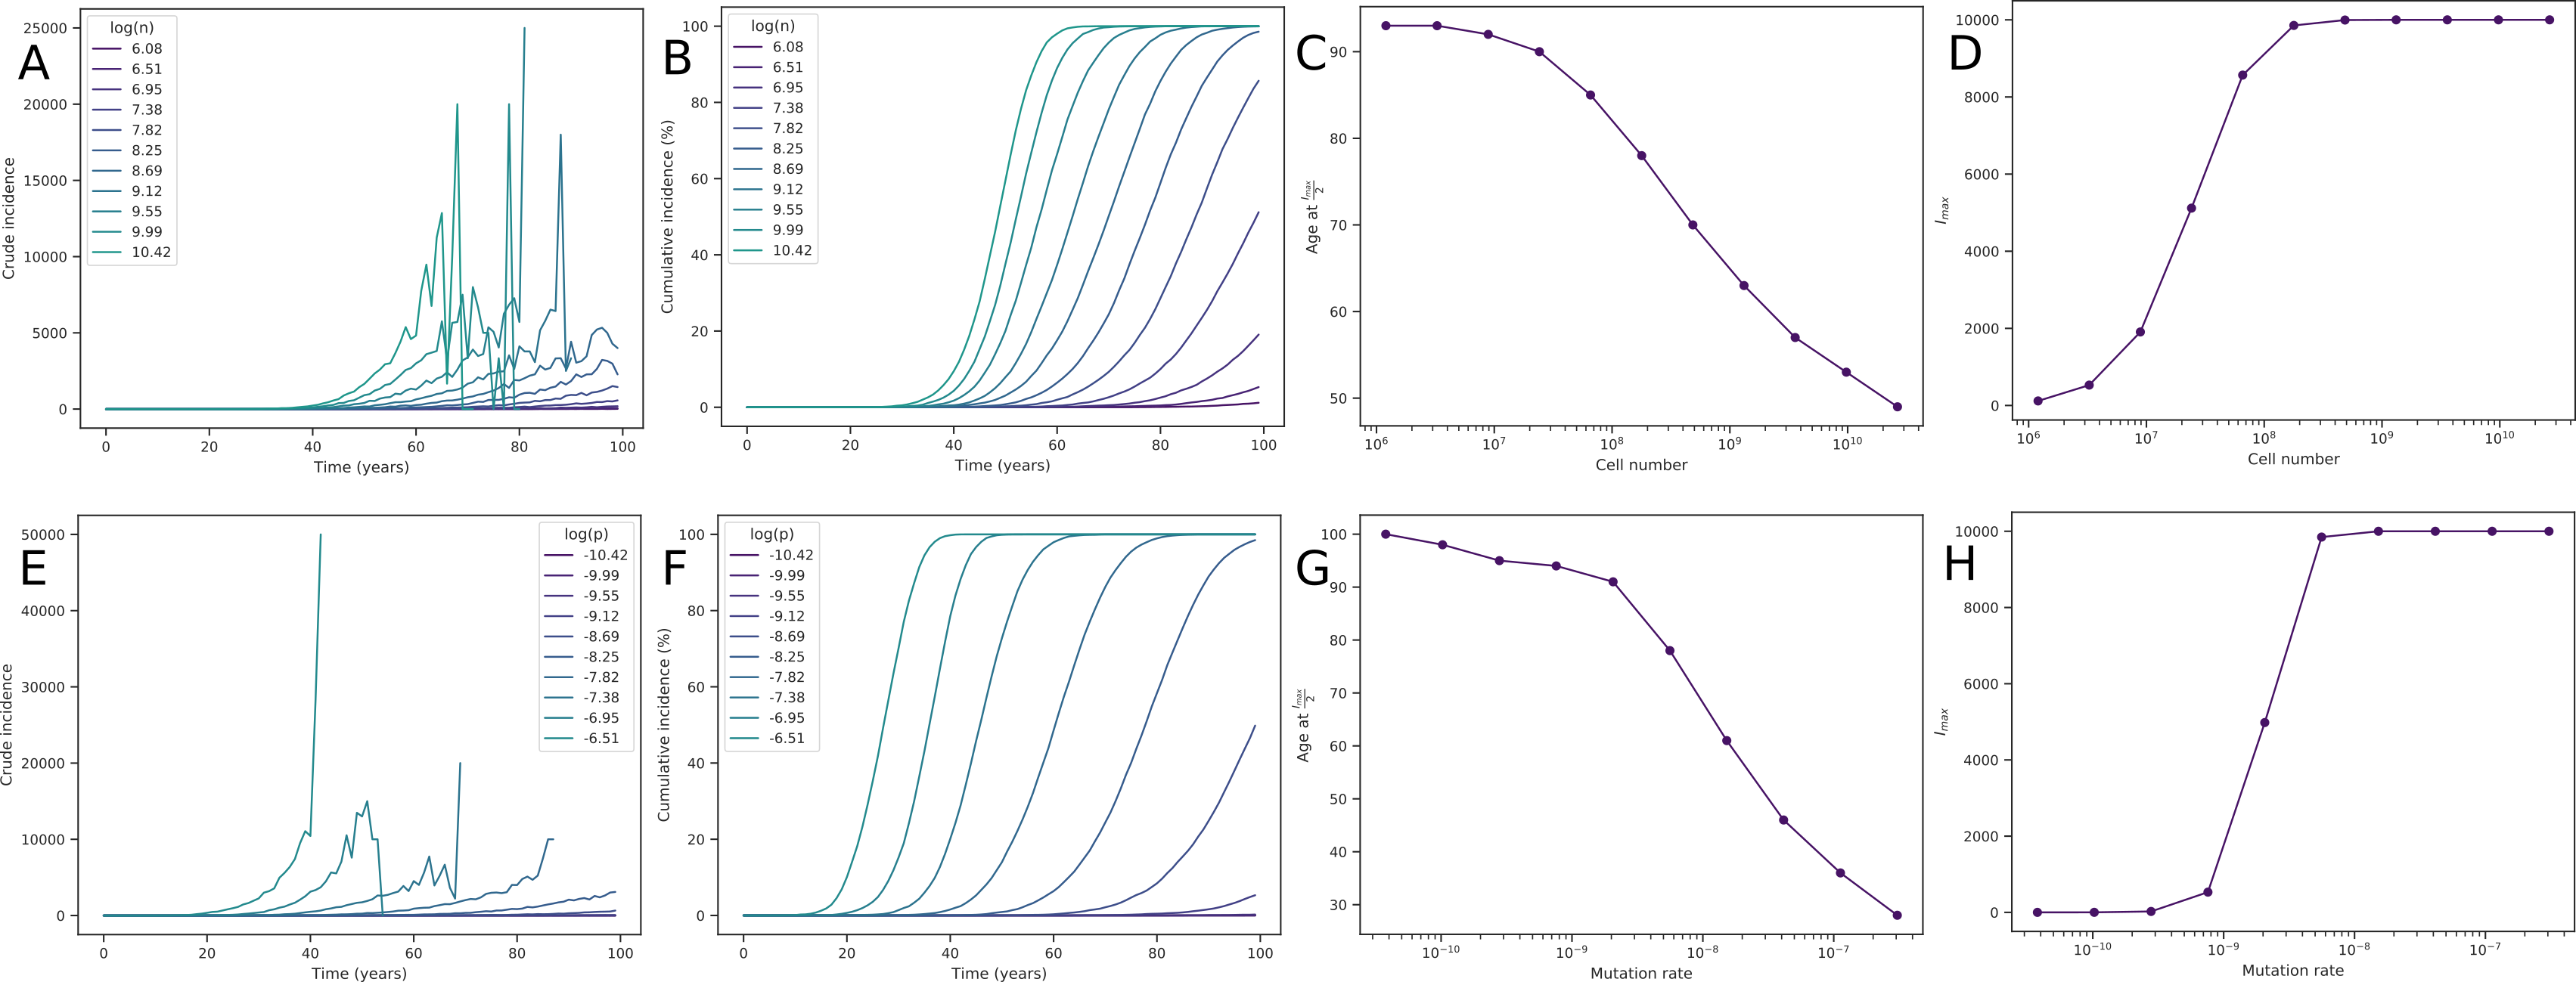
\includegraphics[width=\linewidth]{fig3.png}
	\caption{Incidence patterns from the context-independent selection model over the range of (A-D) $n$, and (E-H) $p$. From left to right in each row, the plots are of (A, E) age-specific crude incidence per 100,000 vs age, (B, F) cumulative incidence (\% of simulated population) vs age, (C, G) age at which half the maximum incidence is reached vs $n$ or $p$, and (D, H) the maximum cumulative incidence, $I_{max}$ vs $n$ or $p$. Incidence saturates only at 100\%, both with time (B and F), and with $n$ and $p$ (D and H). Inset legends for the age curves are $log(n)$ and $log(p)$ in the top and bottom row respectively. For A-D, $p=5.603*10^{-9}$, and for E-H, $n=1.785*10^{8}$. Growth rates progress linearly in the general form, $g_{i}=0.007*(i+1)$, where $i=0,...,k$ and $k=5$.}
	\label{fig3}
\end{figure*}

\begin{figure}[tbhp]
	\centering
	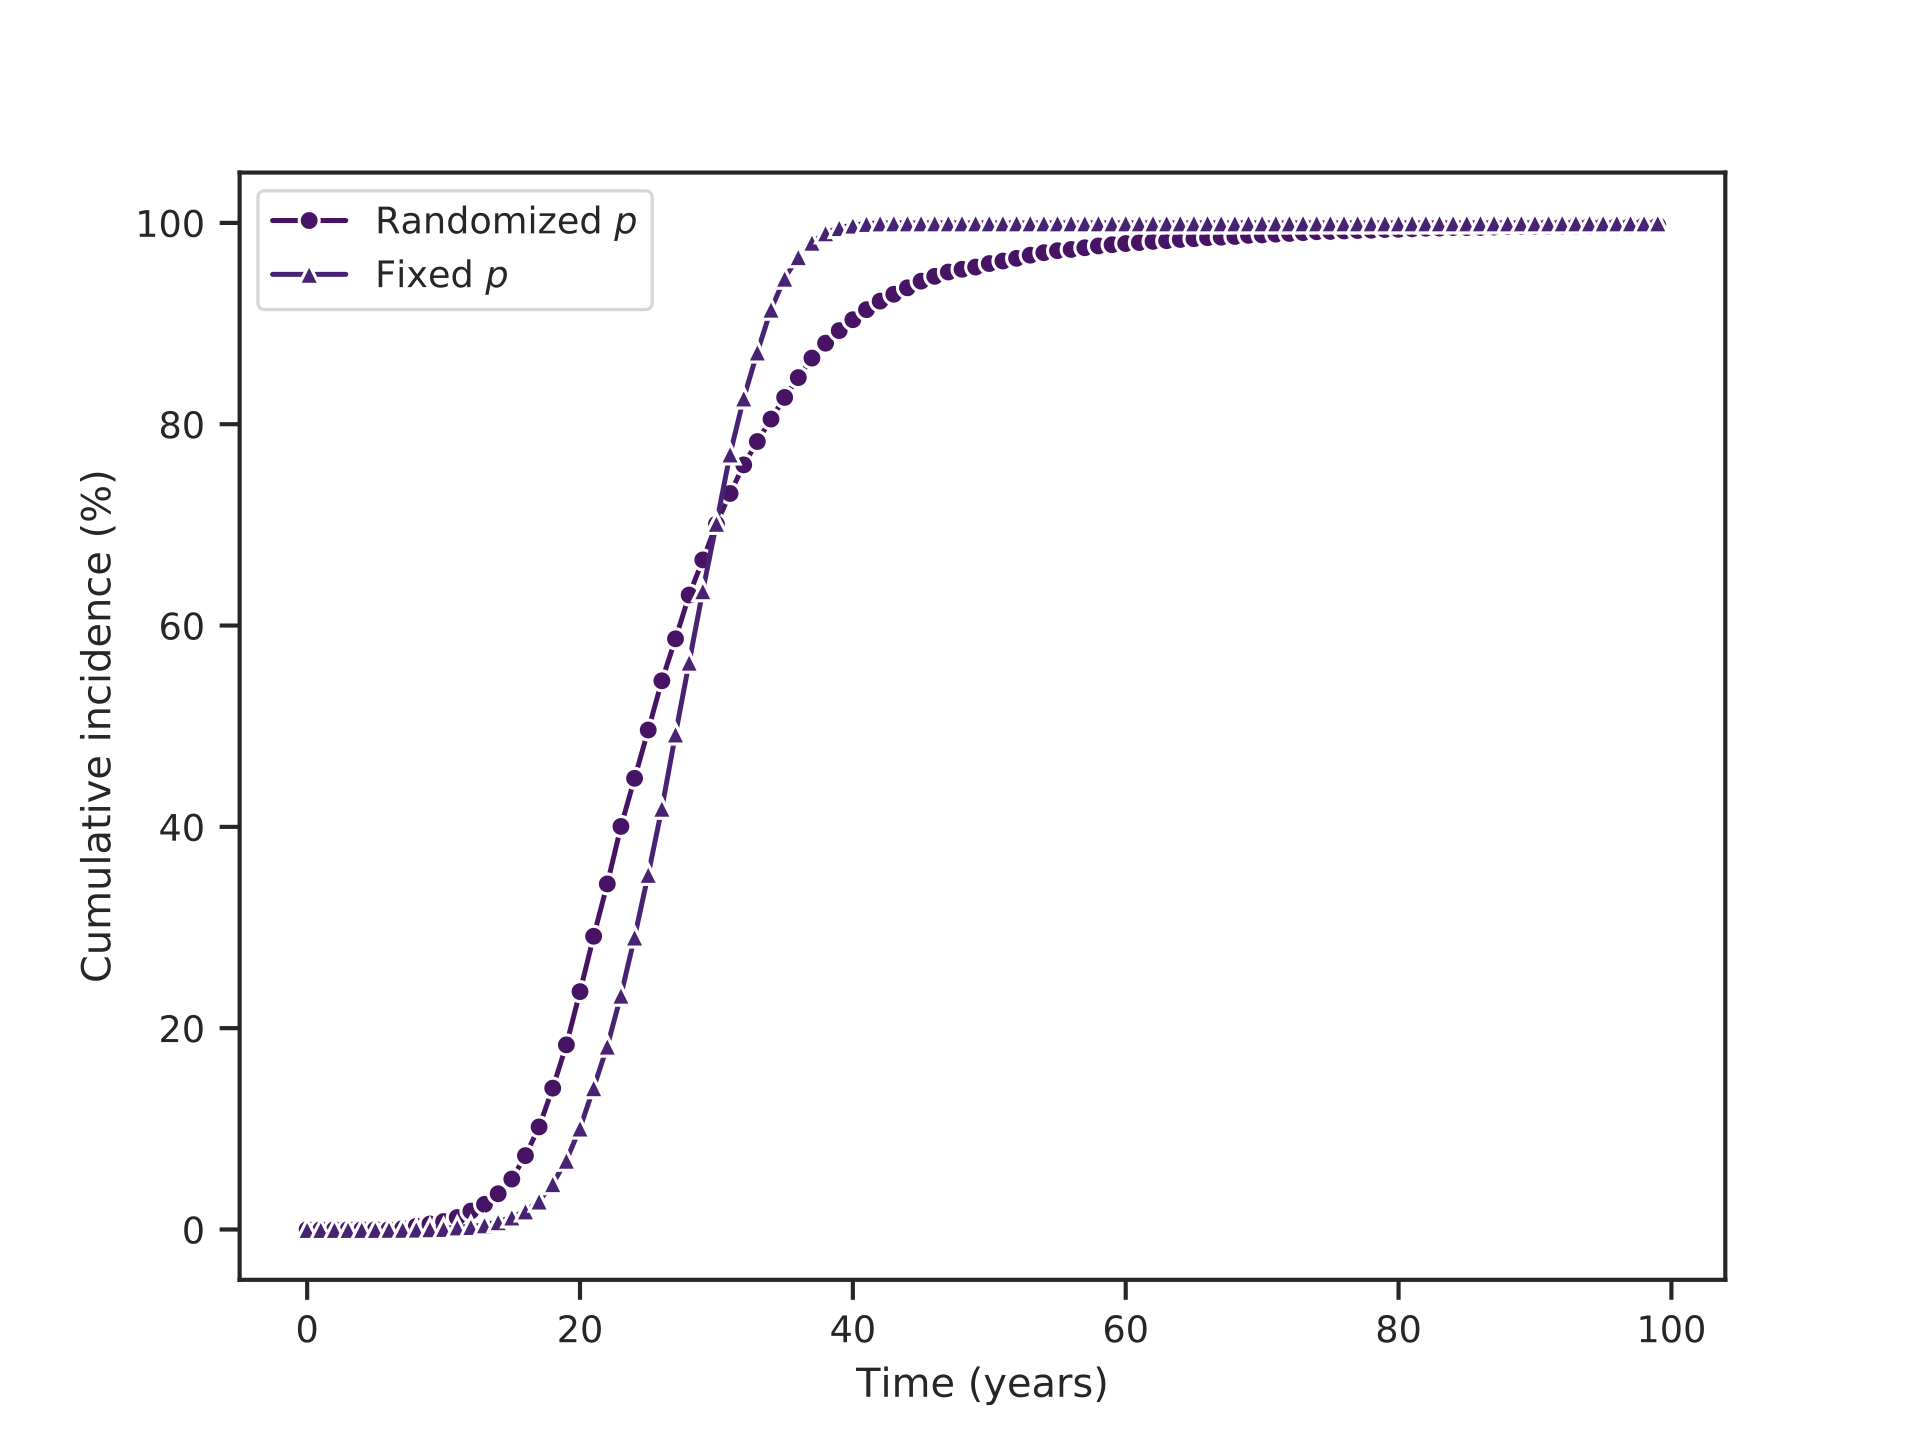
\includegraphics[width=\linewidth, keepaspectratio=true]{fig4.png}
	\caption{Cumulative incidence (\% of simulated population) with randomized vs fixed $p$ for the population in the context-independent selection case; giving a distribution to $p$ does not reduce the saturation of incidence from 100\%, but slows the transition to 100\%. In the randomized case, $p$ values were drawn from a uniform distribution with range $[3.775*10^{-11}, 3.06*10^{-7}]$ and mean, $\overline{p} = 4.17*10^{-7}$, while for the fixed case, $p=3.06*10^{-7}$; for both, $n=1.785*10^{8}$ and $k=5$.} 
	\label{fig4}
\end{figure}

As opposed to the context-independent selection model, the context-dependent model produces a saturating trend in cumulative incidence that begins to saturate at a level much lower than 100\% (Figure \ref{fig5}). This is an important feature of the context-dependent model, as it allows the model to generate more realistic patterns in age-specific cancer incidence. The saturation occurs because propensity for clonal expansion varies across individuals; cancer progression occurs very quickly in some individuals, and not at all in others. Of the three models analysed so far, only the context-dependent model captures a trend similar to the late-life decline observed in many cancers in humans, as the crude incidence curves in Figure \ref{fig5}A and E show. It is also important to note that cancer incidence increases progressively over several orders of magnitude of both $n$ and $p$, as opposed to the thresholds observed in earlier models (Figure \ref{fig5}C and G).

\begin{figure*}[tbhp]
	\centering
	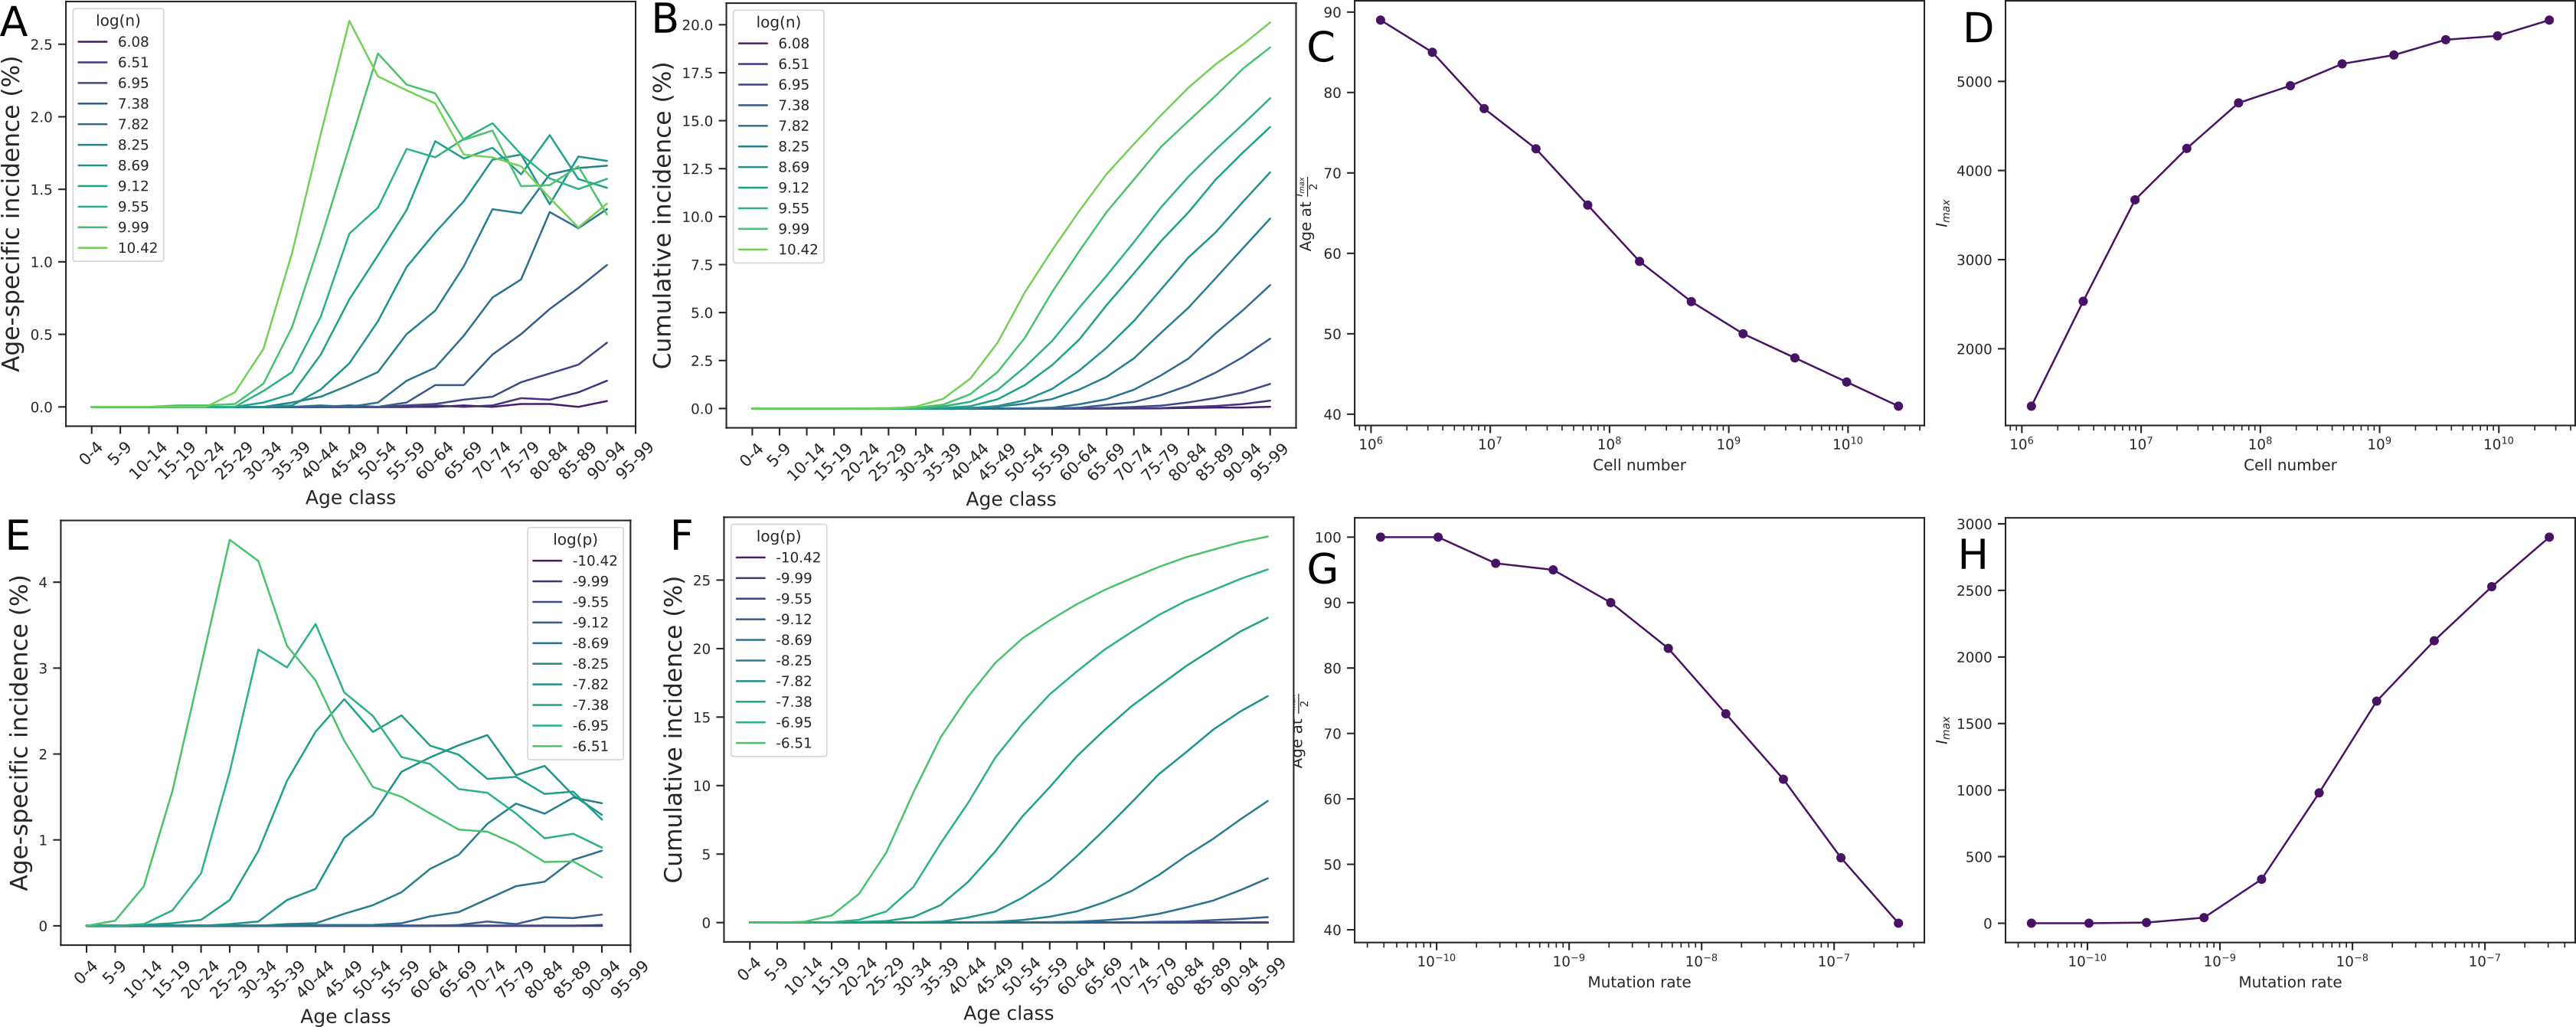
\includegraphics[width=\linewidth, keepaspectratio=true]{fig5.png}
	\caption{Incidence patterns from the context-dependent selection model over the range of (A-D) $n$, and (E-H) $p$. From left to right in each row, the plots are of (A, E) age-specific crude incidence per 100000 vs age, (B, F) cumulative incidence (\% of simulated population) vs age, (C, G) age at which half the maximum incidence is reached vs $log(n)$ or $log(p)$, and (D, H) the maximum cumulative incidence, $I_{max}$ vs $n$ or $p$. As opposed to Figure \ref{fig3}, cumulative incidence saturates much below 100\%, both with time (B and F), and with $n$ (D), when $g$ is randomized in the population. Note that randomization of $p$ alone in the population does not reproduce these patterns (Figure \ref{fig4}). Inset legends for the age curves are $log(n)$ and $log(p)$ in the top and bottom row respectively. For A-D, $p=5.603*10^{-9}$, and for C-H, $n=1.785*10^{8}$. Insets for the incidence curves show $log(n)$ and $log(p)$ in the top and bottom rows respectively. Growth rates progress linearly from $g_{0}=0.007$ to $g_{k}=0.007*\mu$, where $\mu$ is normally-distributed random variable with $\overline{\mu}=3$ and $\sigma=5$, and $k=5$.}
	\label{fig5}
\end{figure*}


\section{Sensitivity of predictions}

Randomizing $k$ in the range, [2, 10] \cite{Martincorena2017}, the nature of the relationships did not change qualitatively, although $k$ affected the age of cancer onset (Supplementary figures, \ref{figS2.1}-\ref{figS2.4}). As different types of cancers may have different $k$ \cite{Nunney2015}, the effects of $n$ and age on incidence trends could also change correspondingly. 

This is also relevant to the study of similar patterns that do not show up at the whole population level, but may become apparent if the population stratified by the number of driver mutations, which in turn is known to vary across cancer types.

To test the assumption of a normal distribution for $\Delta_{g}$, we reevaluated the predictions of the context-dependent selection model for a Gumbel- and uniformly-distributed $\Delta_{g}$ progression. We find that the shape of the distribution does not affect the saturation of cumulative incidence, or the late-life decline in age-specific incidence predicted by the model, although the shape of the age curve changes (Supplementary material, \ref{S1 Figures}).

\section{Discussion}

\begin{table*}[tbhp]
\centering
\begin{threeparttable}
\begin{tabular}{p{5cm}p{4cm}p{4cm}p{3.5cm}p{7cm}}
\textbf{Epidemiological observation} & ``Bad luck'' & Context-independent selection & Context-dependent selection \\
\hline
\textbf{Total incidence across cancer types does not exceed 30\%} & Saturation at 100\% only & Saturation at 100\% only & Saturation<100\% possible \\
\textbf{Age-specific incidence decreases in old age for several cancers} & No late-life decline & No late-life decline & Late-life decline predicted \\
\textbf{Incidence vs $n$} & Sharp threshold saturating at 100\% & Strong threshold saturating at 100\% & Progressive increase over several orders of magnitude \\
\textbf{The phenomenon of non-mutagenic carcinogens} & No explanation offered & No explanation offered & Act through $\Delta_{g}$ distribution \\
\textbf{Peto's paradox-cancer risk saturates with $n$} & Evolved cancer defences & Evolved cancer defences & Cancer incidence not mutation-limited \\
\hline
\end{tabular}
% \begin{tablenotes}
% \item[1] \small{Extrinsic mechanisms like evolved cancer defences must be invoked.}
% \end{tablenotes}
\caption{Summary of model predictions vs epidemiological trends}
\end{threeparttable}
\label{Table 1}
%\addtabletext{nomenclature for the TSs refers to the numbered species in the table.}
\end{table*}

%Returning to the epidemiological patterns in the introduction, we now review the predictions of the three models. The ``bad luck'' model predicts a strong threshold of cancer probability with $n$, $p$ and with age. In all three cases, incidence increases in a roughly sigmoid fashion, and saturates only at 100\% incidence. This is also broadly true of the context-independent selection model, which similarly fails to capture the saturation of incidence at around 30\% in real populations, along with the late-life decline in age-specific incidence observed in several cancer types. Along the same lines, the sharp threshold relationships from both of these models of incidence with both $n$ and $p$ stand in clear contrast to real data. As stated earlier, the relationship between incidence and cell number is claimed to be linear by man in the field \cite{Tomasetti78, Tomasetti2017}. While it remains to be conclusively determined if this relationship indeed is linear or non-linear, there is sufficient basis to reject the threshold prediction from the ``bad-luck'' and context-independent selection model. Regardless of whether we assume linearity over a large range of $n$, or general non-linearity, the actual relationship is still a progressively increasing function of incidence with $n$ where the first two models predict a strong threshold effect. While a similarly detailed look is not possible with current data for the relationship of incidence with $p$, there is again sufficient basis to reject a sharp threshold and/or 100\% incidence as predicted by the ``bad luck'' and context-independent models.

%On all these counts, we see that the context-dependent selection offers much more realistic predictions for the relationship of incidence with $n$, $p$ and age. It can produce saturation of incidence at around observed rates in real populations, the observed late-life decline in incidence, and more realistic relationships with $n$ and $p$. It has also indicated interesting effects of the number of oncogenic mutations required for cancer. While it is expected that higher $k$ increases the time taken for cancer onset, the value of $k$ is also seen to modulate how strongly $n$, $p$ and $g$ affect the time to cancer onset, particularly in the moderate to higher range of $k$. This is an important detail that pan-cancer analyses of incidence trends must take note of. For small values of $k$, $n$ does not affect incidence dynamics, but $g$ and $p$ do. The context-dependent model also offers potential explanations for the late-life decline in age-specific incidence. In the model, we see that cancer incidence is determined to a large extent by $g$, suggesting a selection-limited process. Late-life incidence in the model comes from a slow growth rate progression across mutations, and a late-life decline can therefore be described in terms of the distribution of the growth rate progression. In a population where slow growth rate progression for mutants is rare, organisms with active mutagenesis progress to cancer relatively earlier in life, and cancer is rarer later in life. It becomes important therefore, to consider the local or evolutionary factors underlying such a temporal pattern of mutation accumulation. 

Table \ref{Table 1} compares the prediction profile of the three models discussed so far. On the whole, the better prediction profile of the context-dependent model stems from the distribution of $g_{i}$ in the population, and this has interesting implications for the kind of causal factors that are important in explaining cancer etiology. One of these implications concern the mutation-centric thinking that represents the mainstream thinking in cancer biology. For instance, several growth factors and hormones are known to increase cancer risk, not the least of which is insulin, without increasing the basal mutation rate or the cell number. The action of such ``non-mutagenic carcinogens'' is not compatible with a mutation-centric approach to carcinogenesis. We propose instead that non-mutagenic carcinogens could act by altering $\Delta_{g}$.
Similarly, late-life incidence in the model comes from a slow growth rate progression across mutations. By extension, the late-life decline comes from the left-hand tail of the $\Delta_{g}$ distribution, with zero or negative progression in some individuals. It becomes important therefore, to consider the local or evolutionary factors underlying such a temporal pattern of mutation accumulation.
This line of thinking can also be extended to address Peto's paradox. It is not a new argument that Peto's paradox can be explained by invoking selection \cite{Caulin2011,Noble2015,Tollis2017b}. The results from our model in fact reinforce the notion that somatic evolution of cancer is largely selection-limited, rather than mutation-limited, which explains why cancer risk does not increase in proportion with cell number and/or body size. Moreover, our analysis introduces the additional dimension of population-level variation in cancer propensity as part of the explanation of Peto's paradox.
This variation in selection could be attributed to the micro-environment in the tumour or pre-cancerous niche, and includes all the factors that determine the selective advantage of oncogenic or pre-cancerous mutants. As mentioned earlier, empirical evidence of such context dependence has been accumulating on multiple fronts \cite{Hansen2000,Pietras2010,Hanahan2012,Cabarcas2011a}. \textit{In vitro}, the IGF-II concentration in culture media is found to markedly alter the selective advantage of an IFG-II over-expressing mutant in cell competition \cite{Archetti2015}. Pre-cancerous cell lines across cancer stages also show different growth properties depending on growth factor concentration in the culture medium \cite{Chan2014}. Similar regluatory effects have also been observed for estrogen and progesterone in various cancer types \cite{Haslam2001,Woodward2000,DICKSON1987,Garcia1992}. More recently, experiments have been reported in which behaviourally-enriched environments or physical exercise seemed to show cancer-suppressive effects \cite{Cao2010,Rundqvist2013} that correlate with secretion of particular growth factors. Studies in mice have also shown substantial variation in tumour sizes induced by identical genetic clones across individuals \cite{Rogers2017}, suggesting that context-dependent factors from the microenvironment could play a limiting role in cancer progression. Taken together, these observations suggest interesting avenues of transalational importance for cancer prevention and therapy. An alternative research focus emerges, centered on the microenvironmental factors that drive context-dependent cancer progression. Identifying these factors would lead to novel preventive measures, along with potential implications for therapy.

A composite view of cancer etiology requires not only the incorporation of these, and other complexities in models, but also the comparative testing framework that continues to be rare in cancer literature, barring a few efforts \cite{Frank2007}. The value of such a framework is immense, as it allows for falsification of factors that make predictions contrary to observed data; this falsification is frequently more robust and informative than an indirect confirmation of potential causal factors. With our analysis, we hope to bring this framework back into the mainstream at a time when the availaibility of large-scale data spanning levels of biological organization is better than ever before, from the population to the various cellular ``-omes''. A comparative framework could prove more powerful now, in the context of robust data and computational techniques, and should therefore become a major focus for the cancer modeling effort.

\section*{Acknowledgements}
The authors acknowledge critical input faculty members at the Department of Biology, IISER Pune. We thank Ketaki Bhagwat, Dr. Ruchika Kaul-Ghanekar, Prerna Raina, Dr. Anil Gore, and Dr. Sharmila Bhapat for useful discussions.

\newpage
\printbibliography


\section*{Supporting Information (SI)}
	\renewcommand{\thesubsection}{S\arabic{subsection}}
	\setcounter{subsection}{0} 	

	\subsection{Alternative distributions of $g$}\label{S1 Figures}
		As explained in the main text, we explore the effects of using alternative distributions for the logistic growth rate progression. Figure \ref{figS1.1} shows the effect of a Gumbel-dsitributed progression, and Figure \ref{figS1.2} shows that of a uniformly-distributed progression. We note that the different distributions produce qualitatively the same results as the normal distribution used throughout the main text.

		\renewcommand{\thefigure}{S1.\arabic{figure}}
		\setcounter{figure}{0} 	
		\begin{figure*}[tbhp]
			\centering
			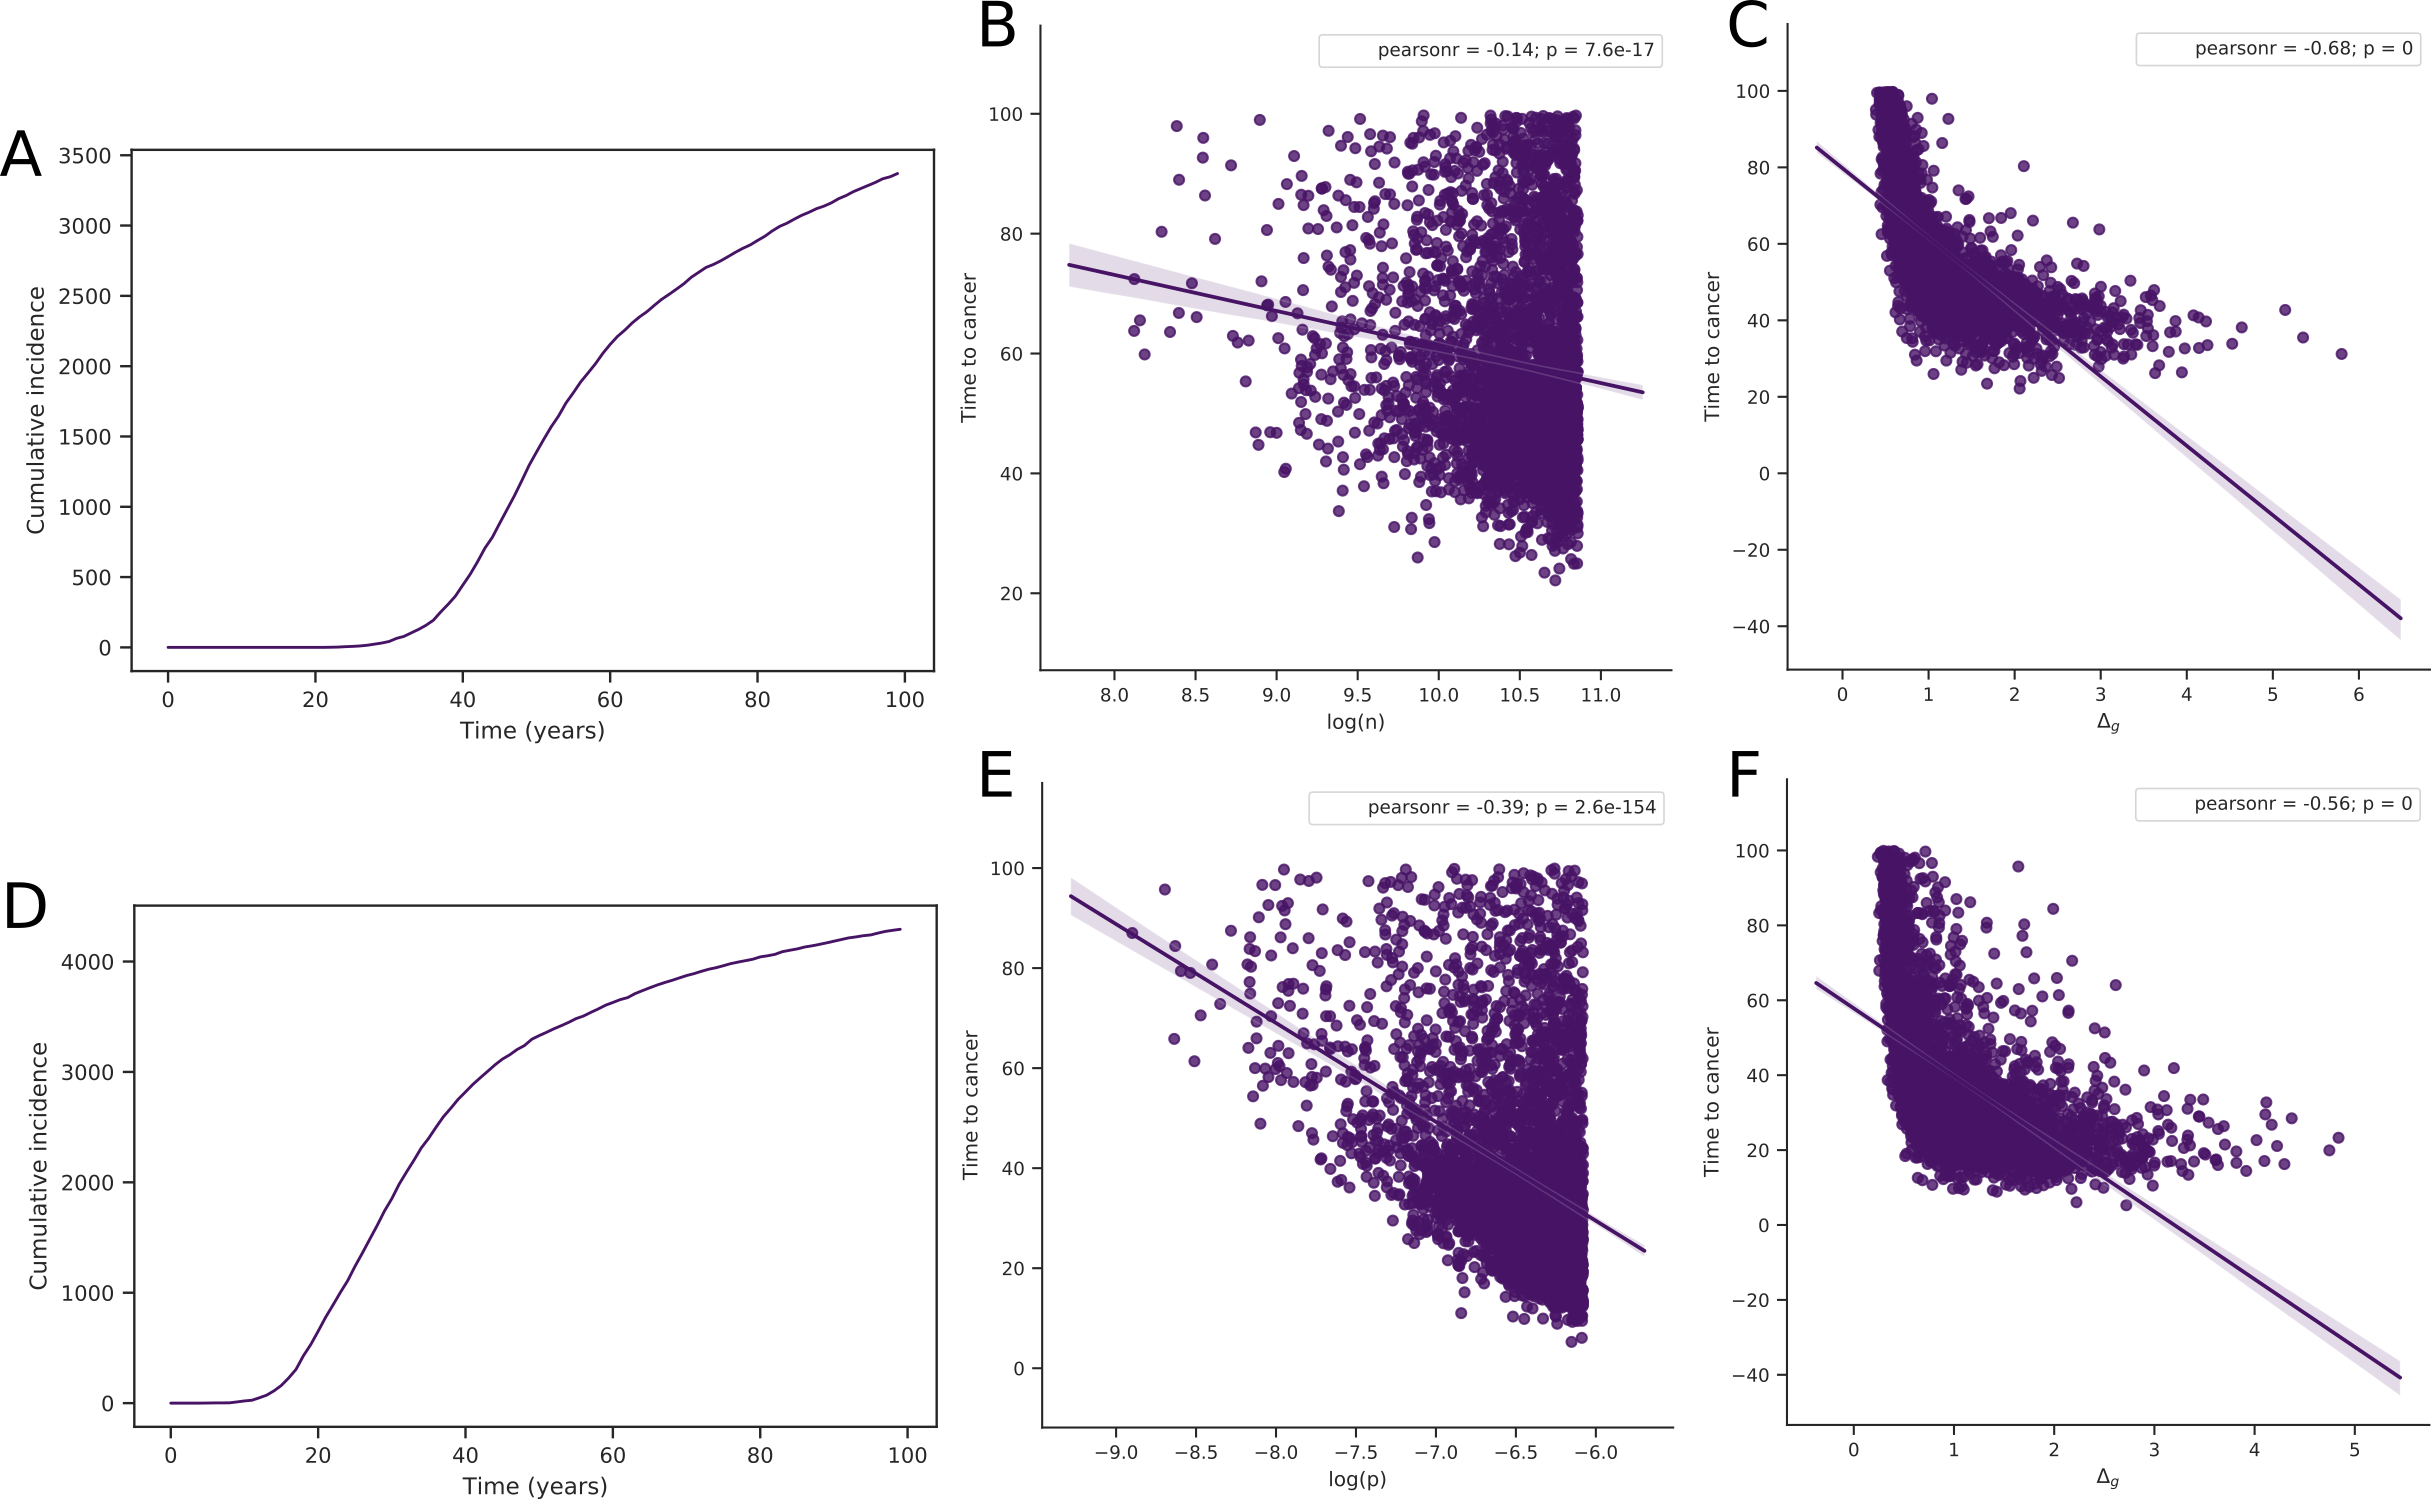
\includegraphics[width=\linewidth, keepaspectratio=true]{figS1-1.png}
			\caption{$g$ modeled by a Gumbel-distributed random variable, $\mu$, with $\overline{\mu}=0$ and $\sigma=3$, co-randomizing $n$ (top row) or $p$ (bottom row), with ranges $[1.203*10^{6}, 2.649*10^{10}]$, and $[3.775*10^{-11}, 3.059*10^{-7}]$ respectively; (A and D) cumulative incidence (\% of simulated population) vs age, and time to cancer vs (B) $log(n)$, (E) $log(p)$, and (C and F) $\Delta_{g}$; $\Delta_{g} = \frac{g_{k}-g{0}}{k}$ and $g_{k} = 0.007*\mu$. For all cases, $k=5$.}
			\label{figS1.1}
		\end{figure*}

		\begin{figure*}[tbhp]
			\centering
			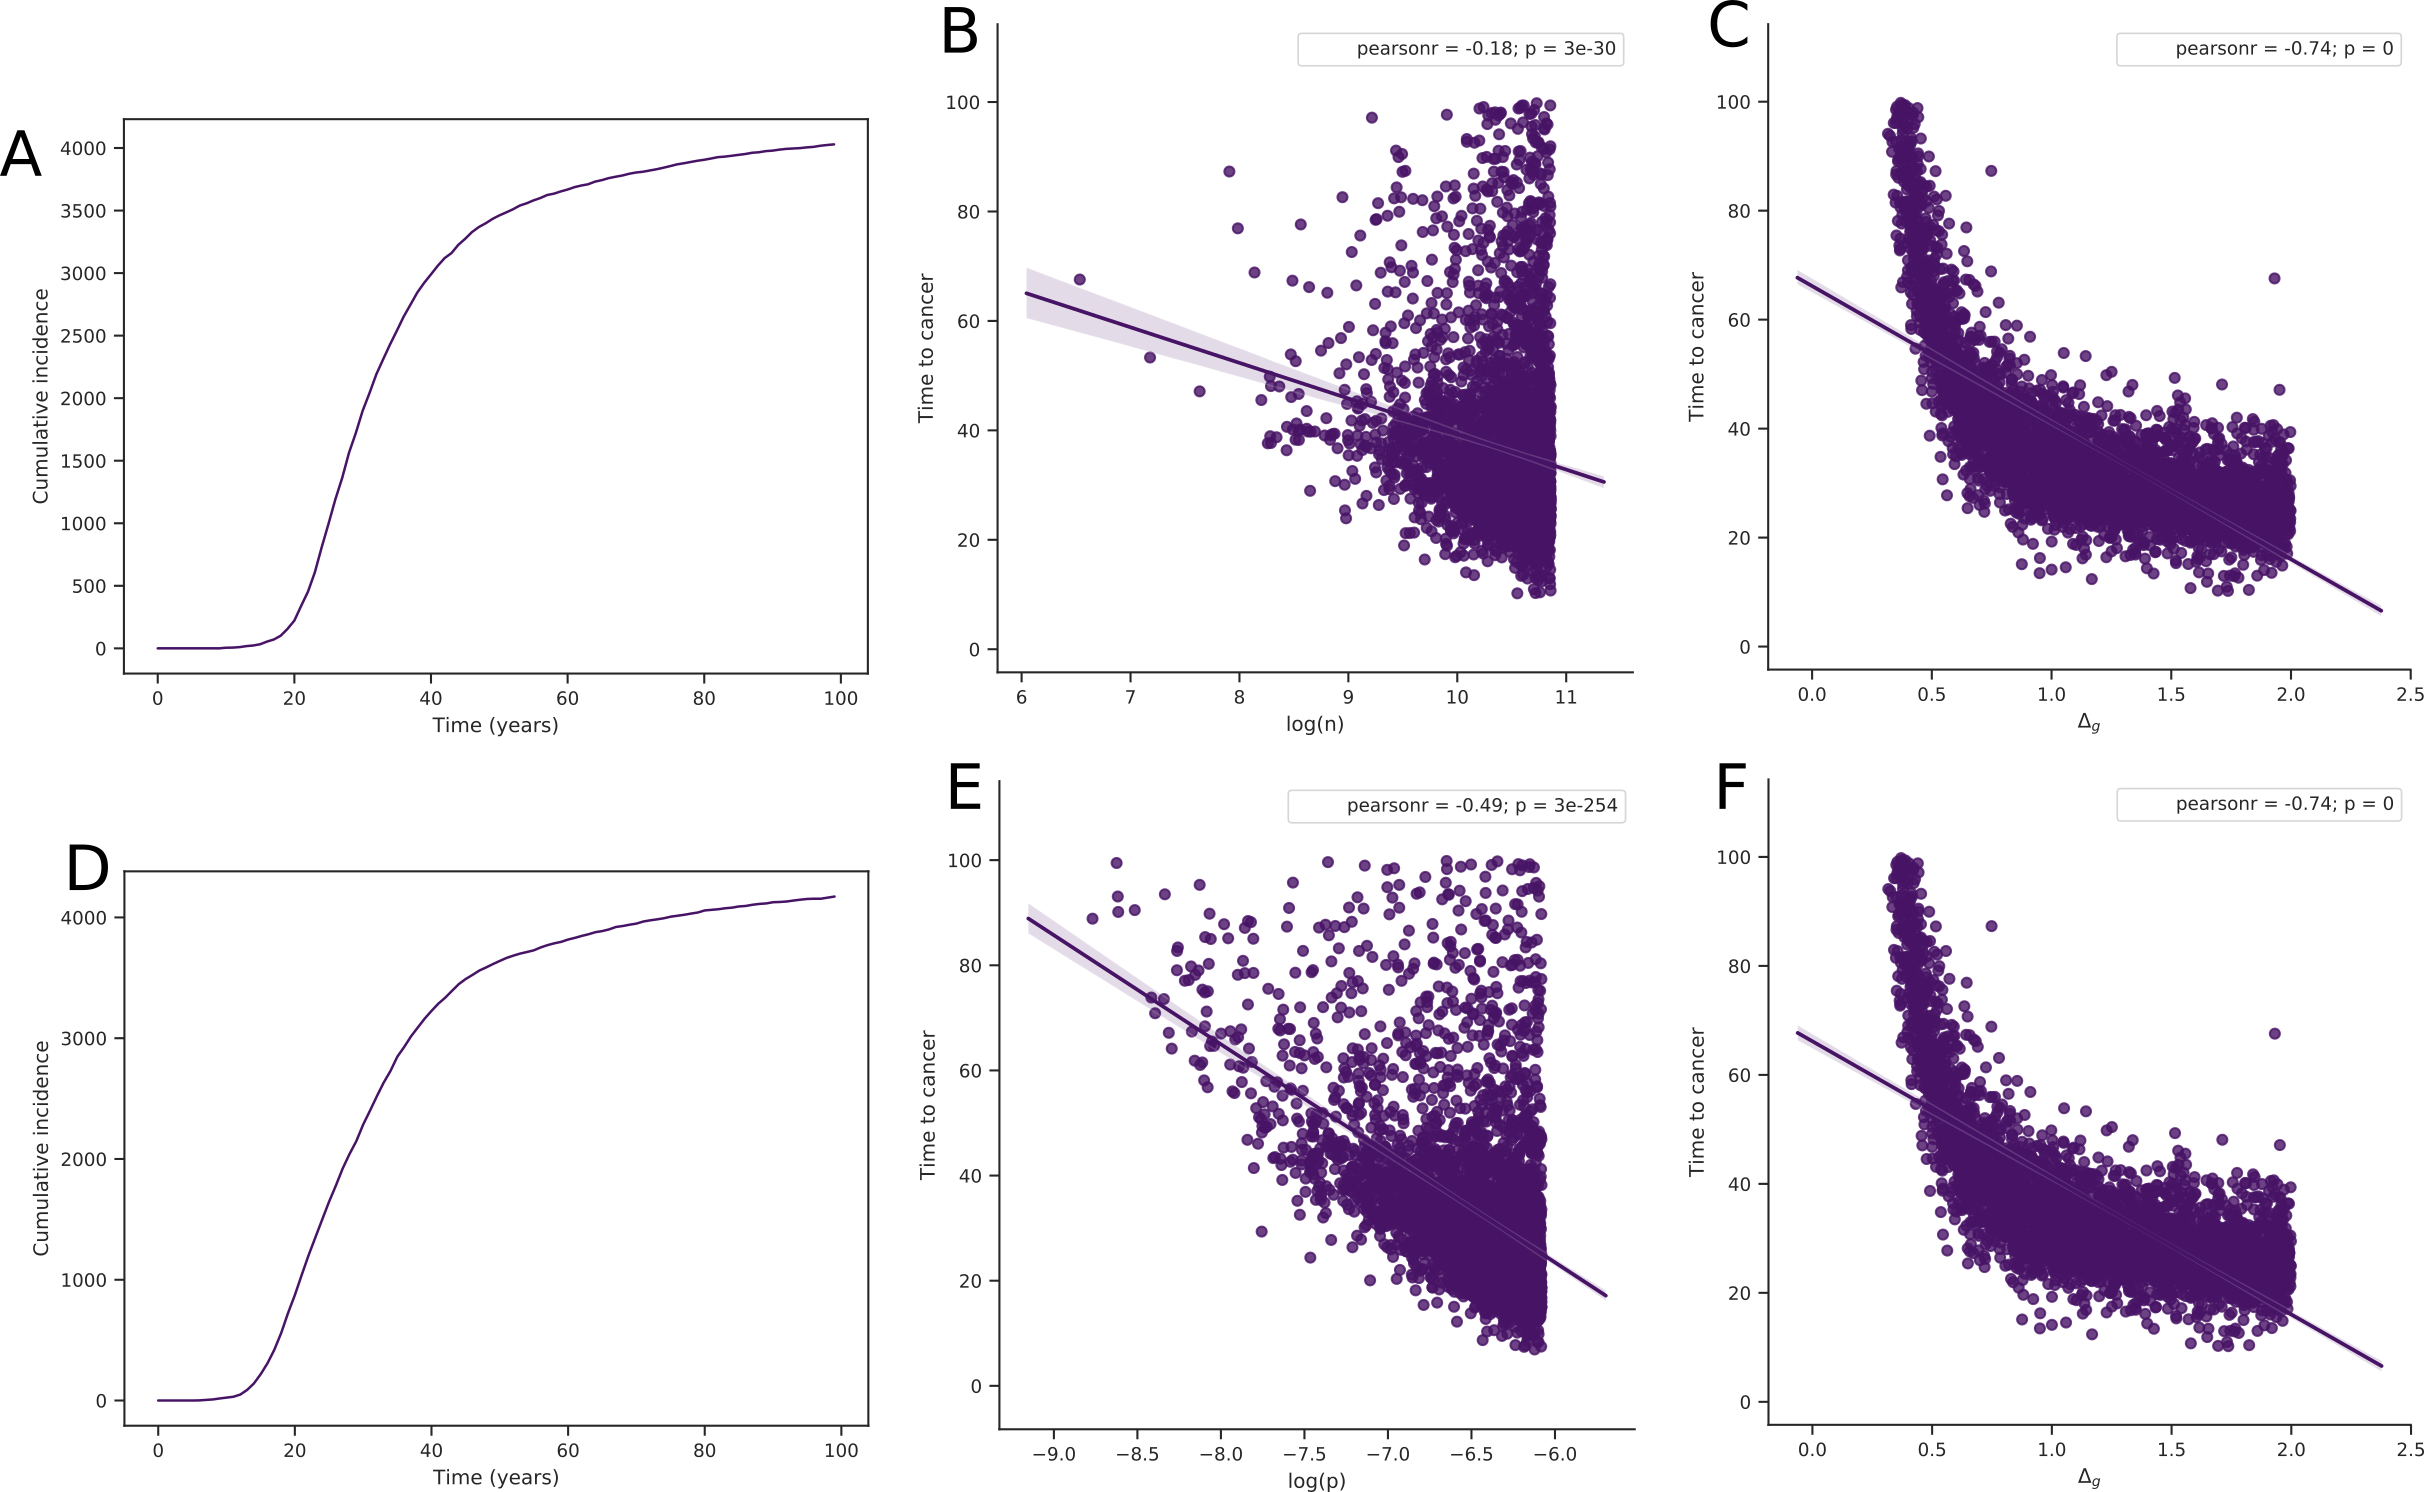
\includegraphics[width=\linewidth, keepaspectratio=true]{figS1-2.png}
			\caption{$g$ modeled by a uniformly-distributed random variable, $\mu$ with range $[-10, 10]$, co-randomizing $n$ (top row) or $p$ (bottom row), with ranges as specified in Figure \ref{figS1.1}; (A and D) cumulative incidence for the simulated population vs age, and time to cancer vs (B) $log(n)$, (E) $log(p)$, and (C and F) $\Delta_{g}$; $\Delta_{g} = \frac{g_{k}-g_{0}}{k}$ and $g_{k} = 0.007*\mu$. For all cases, $k=5$.}
			\label{figS1.2}
		\end{figure*}

	\subsection{Sensitivity of model predictions to $k$}\label{S2 Text}
		\renewcommand{\thefigure}{S2.\arabic{figure}}
		\setcounter{figure}{0}
		\begin{figure*}[tbhp]
			\centering
			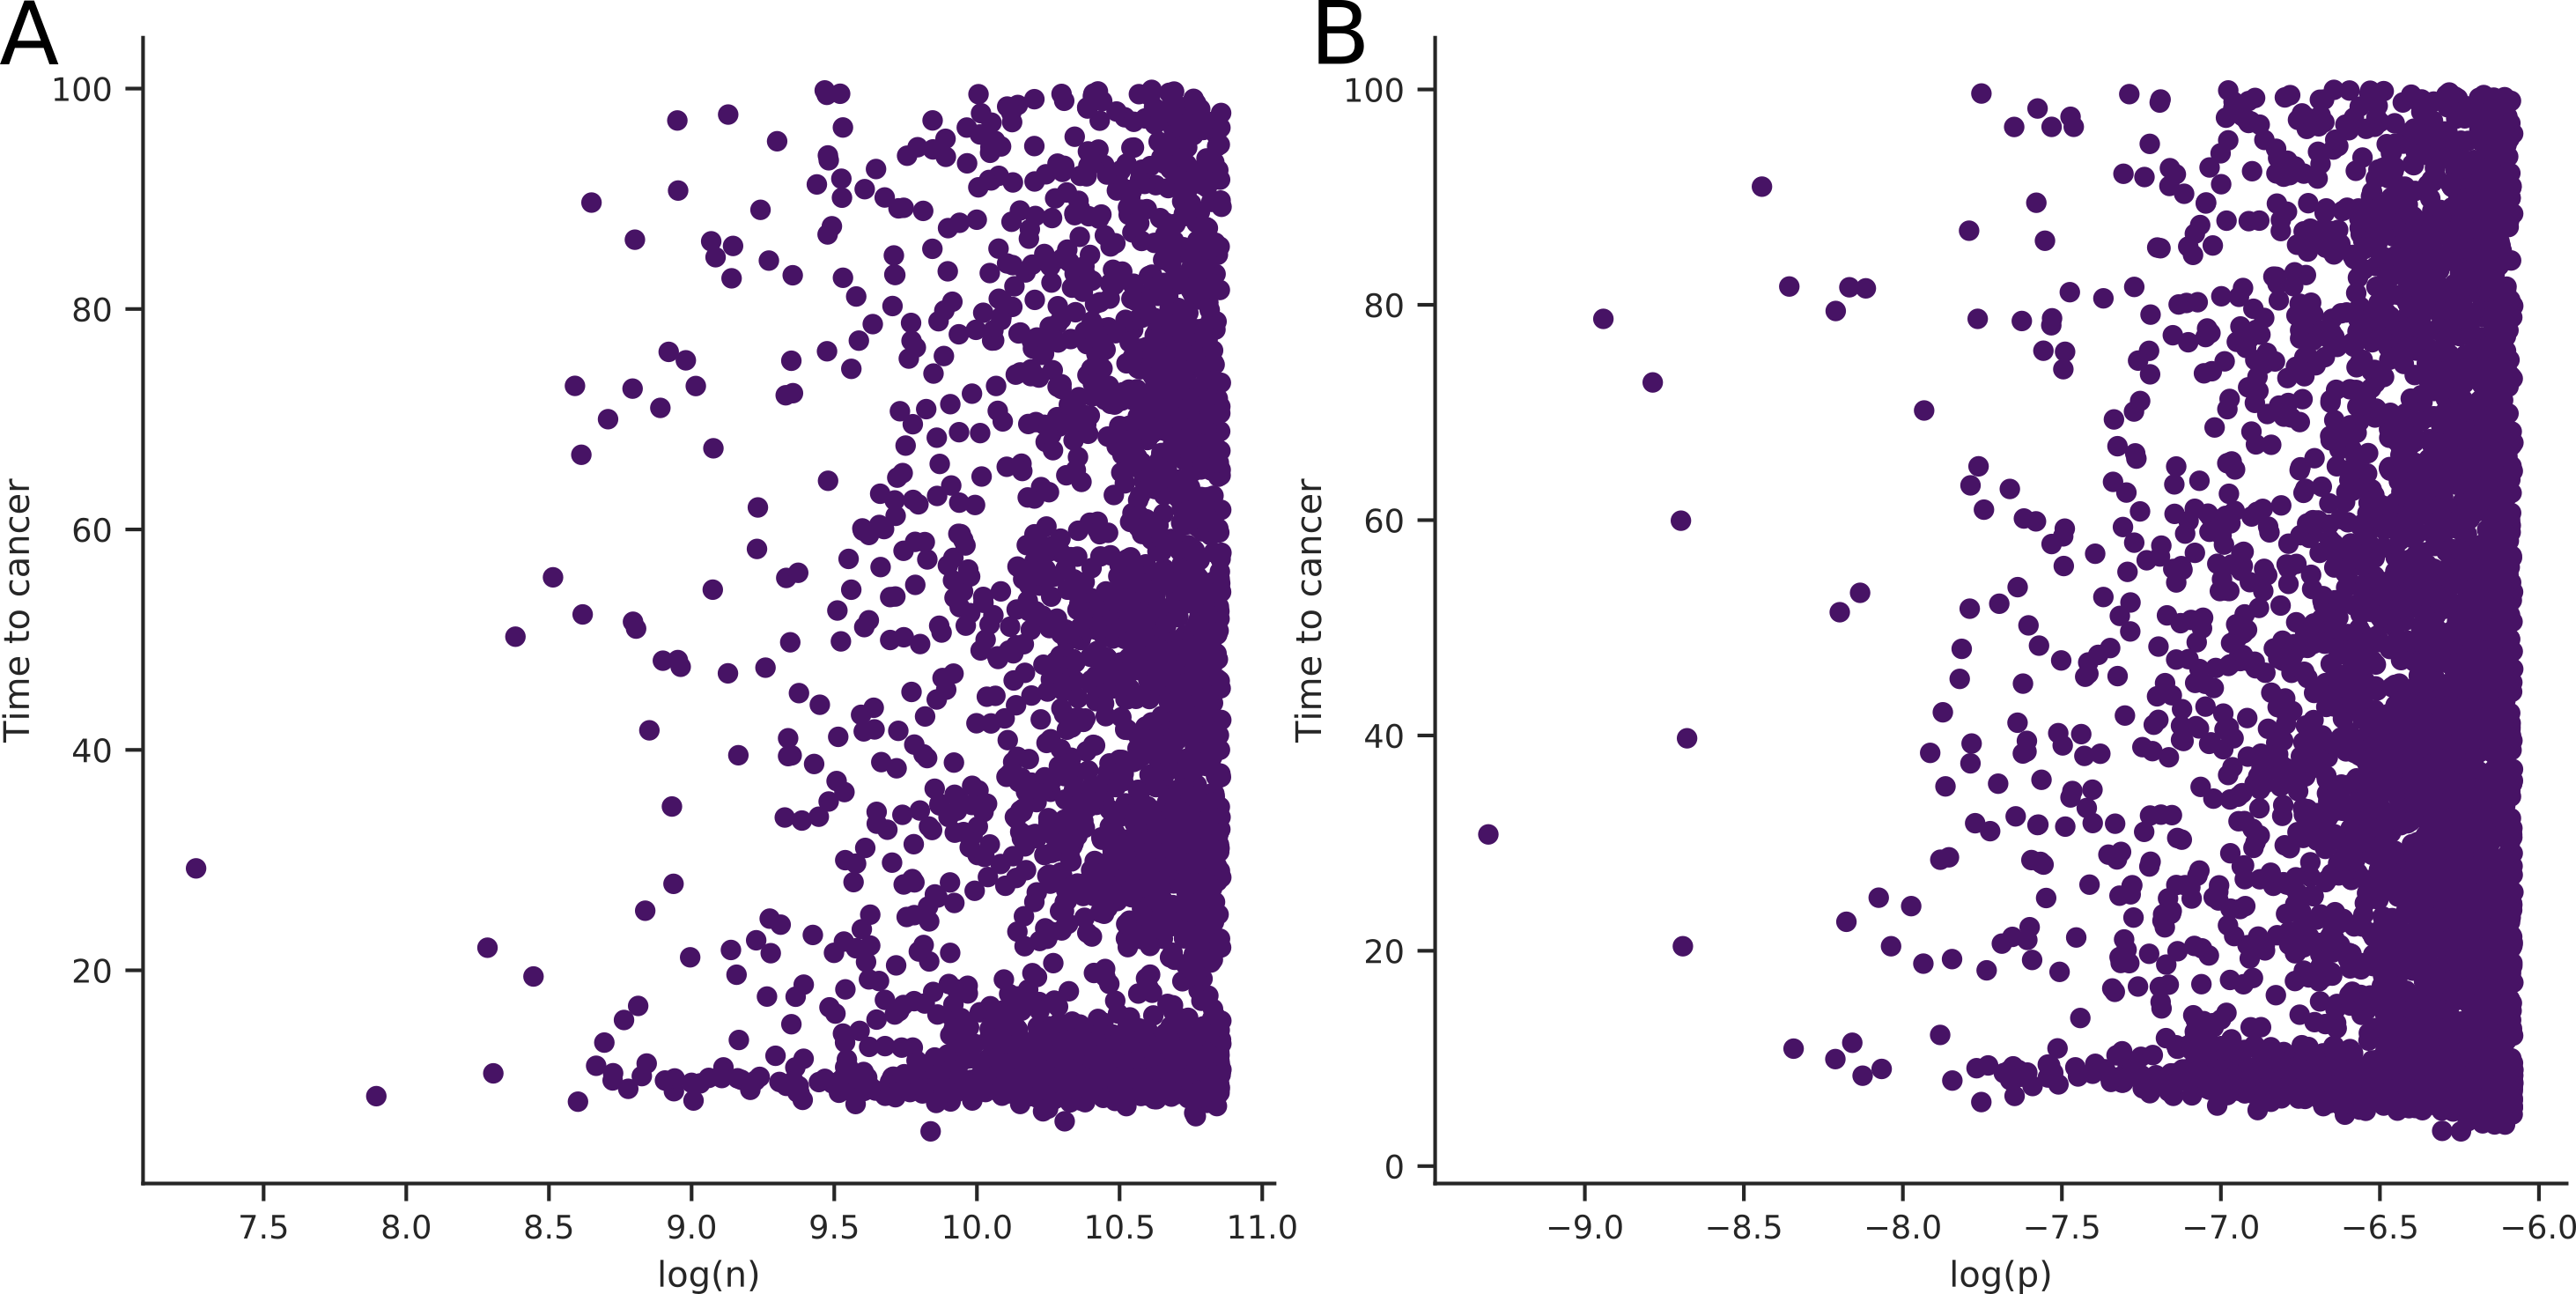
\includegraphics[width=\linewidth, keepaspectratio=true]{figS2-1.png}
			\caption{Effect of randomizing $k$ in the context-independent selection case. The plots are time to cancer onset against $log(n)$ or $log(p)$, with $k$ randomized with (A) $n$, or (B) $p$; when time to cancer is pooled across values of $k$, the association between either $n$ or $p$ is practically non-existent. $k$, $n$ and $p$ were uniformly-distributed random variables with ranges $[0, 20]$, $[1.203*10^{6}, 2.649*10^{10}]$, and $[3.775*10^{-11}, 3.059*10^{-7}]$ respectively; for (A), $p=5.603*10^{-9}$, and for (B), $n=1.785*10^{8}$.}
			\label{figS2.1}
		\end{figure*}

		\begin{figure*}[tbhp]
			\centering
			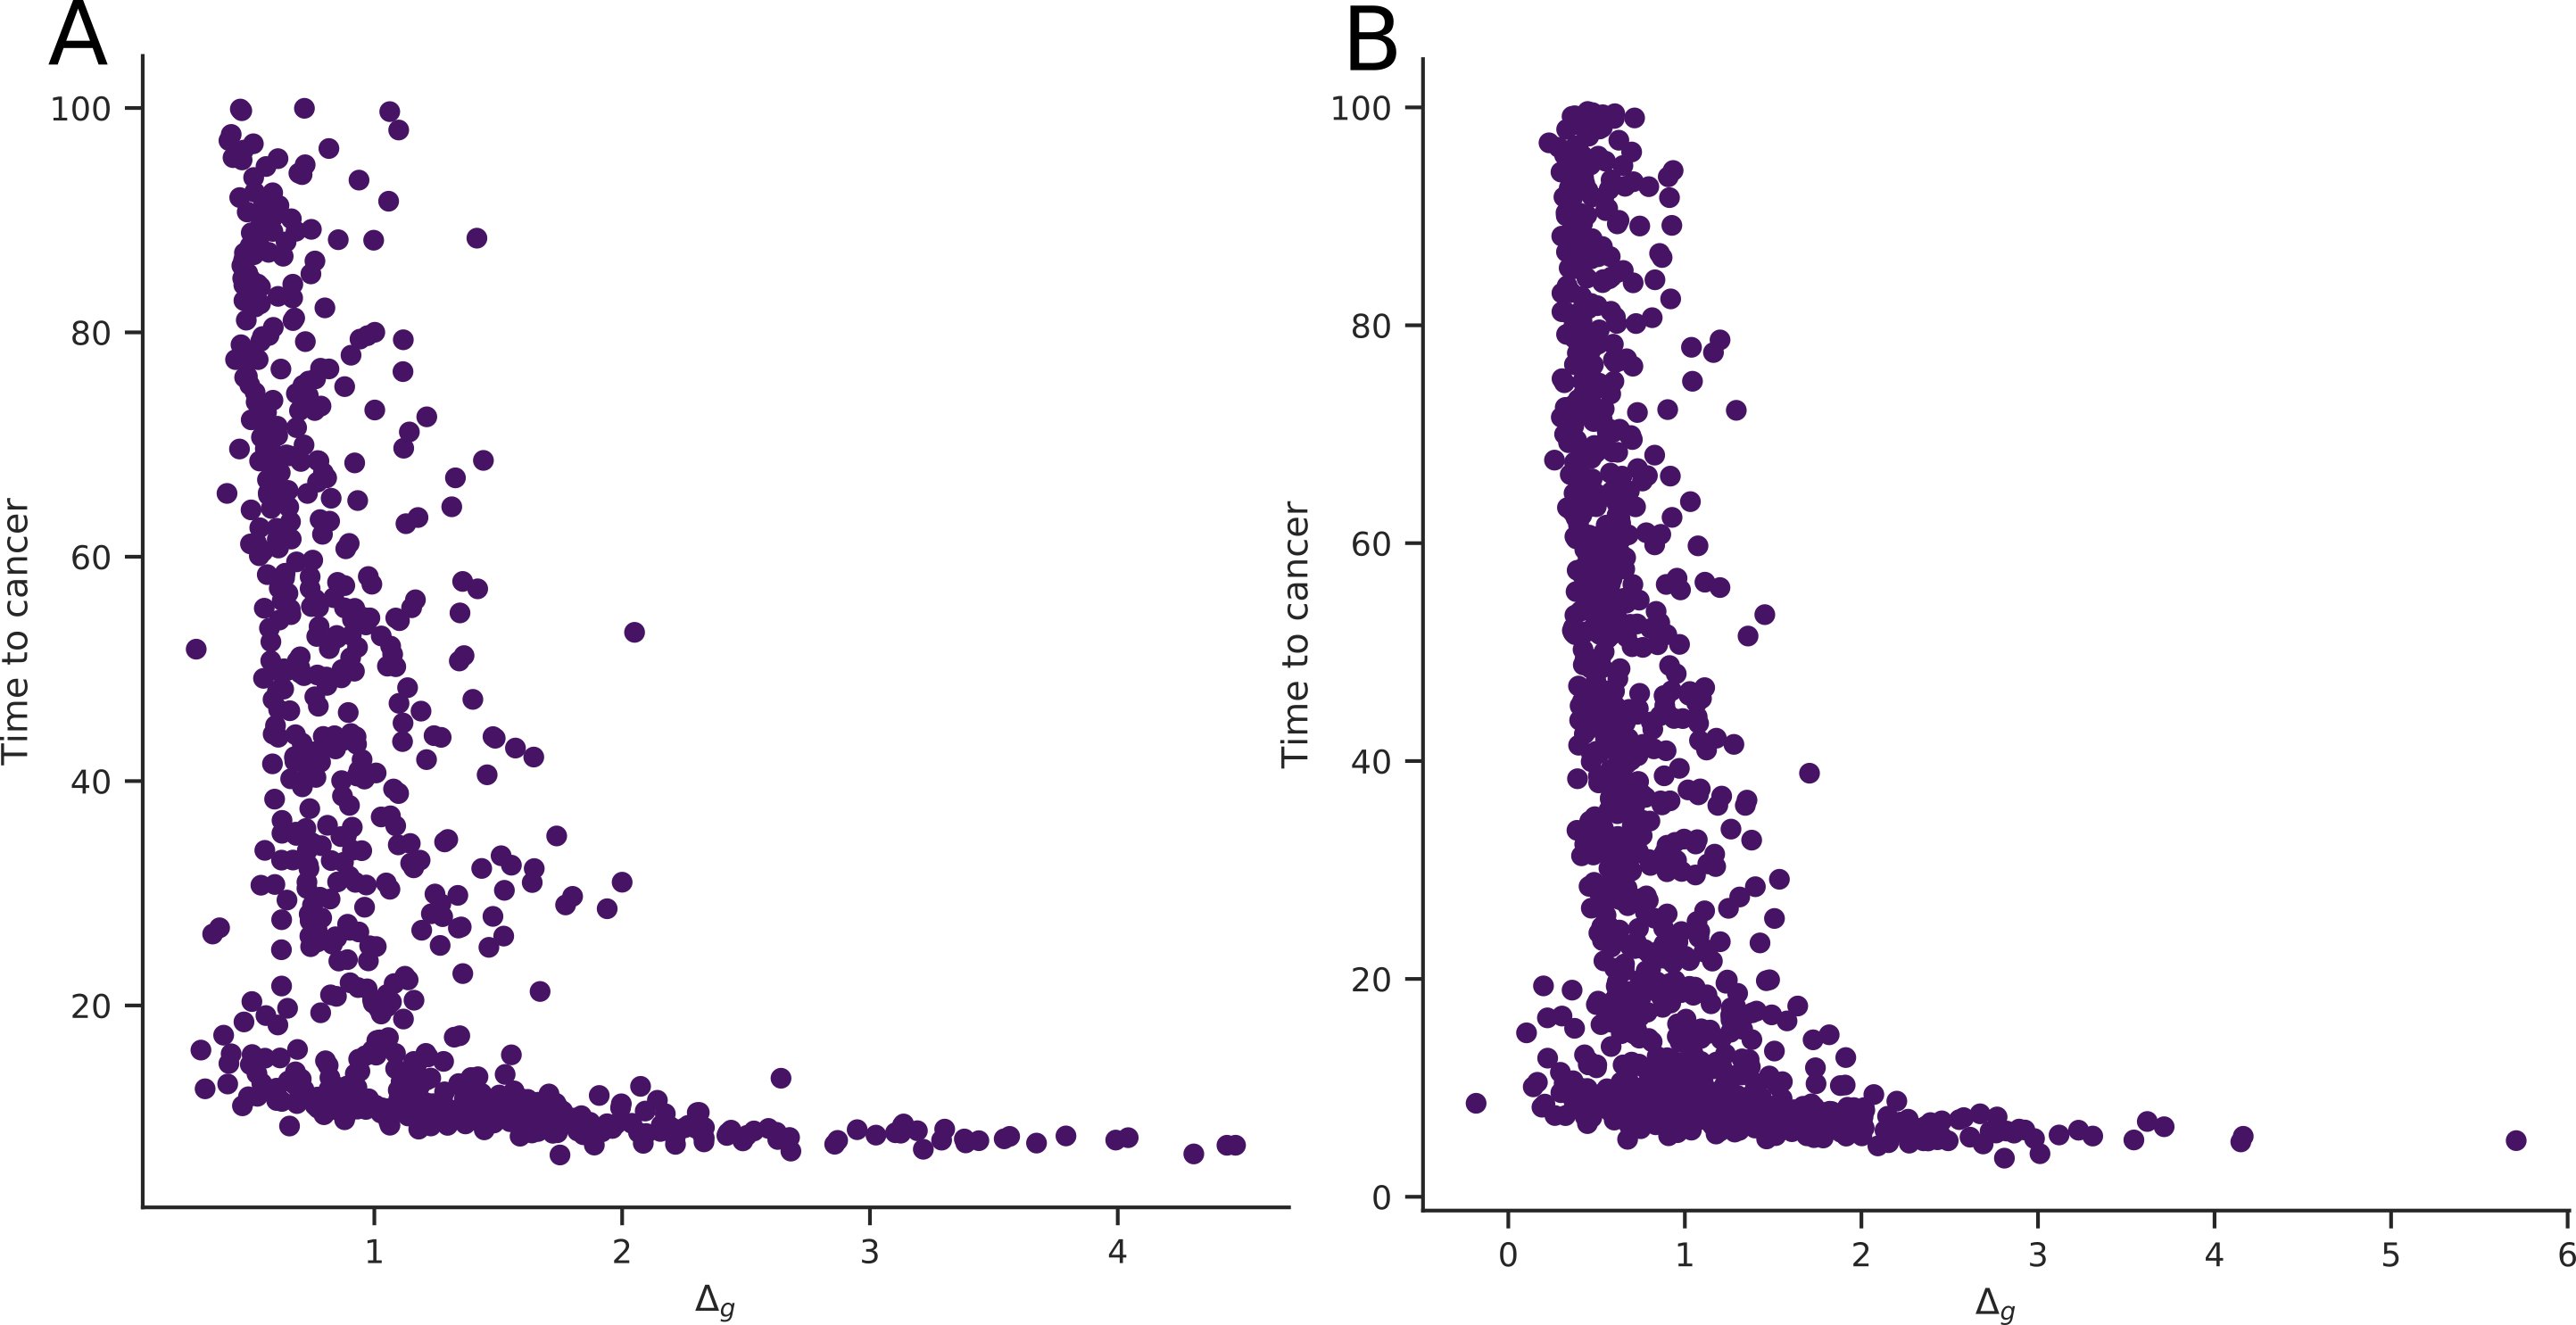
\includegraphics[width=\linewidth, keepaspectratio=true]{figS2-2.png}
			\caption{Effect of randomizing $k$ in the context-dependent selection case. The plots are time to cancer onset against $\Delta_{g} = \frac{g_{k}-g_{0}}{k}$ and $g_{k} = 0.007*\mu$, also randomizing (A) $n$, or (B) $p$; $\Delta_{g}$ measures the rate of the growth rate progression in each individual, and $\mu$ is a normally-distributed random variable with $\overline{\mu}=0$ and $\sigma=3$. As opposed to $n$ and $p$, the association of $\Delta_{g}$ with time to cancer is less affected by $k$. When time to cancer is pooled across all $k$, $\Delta_{g}$'s effect on time to cancer appears distinctly non-linear. $k$, $n$ and $p$ were uniformly-distributed random variables with ranges $[0, 20]$, $[1.203*10^{6}, 2.649*10^{10}]$, and $[3.775*10^{-11}, 3.059*10^{-7}]$ respectively. For (A), $p=5.603*10^{-9}$, and for (B), $n=1.785*10^{8}$.}
			\label{figS2.2}
		\end{figure*}

		As motivated briefly during discussion on model sensitivity, it is important to explore the effect of $k$ on the observed relationships of $p$ and $n$ with cancer incidence. The time taken to cancer onset is a useful parameter in this context as it describes the temporal dynamics of mutation accumulation, while allowing for some limited inference regarding total incidence in the population. If time taken to cancer is largely small, population incidence is likely to be large in the given parameter space, and vice versa.

		Broadly, we find that cancer incidence is significant only up to maximum $k=10$. Increasing $k$ also reduces total incidence and shifts the observed time to cancer to later in life, as expected based on mutation accumulation. We also find that the magnitude of $k$ could modulates the strength of the association with $n$, and to a lesser extent, with $p$. Importantly, the effect of either $n$ and $p$ is apparent only when taken for one value of $k$ at a time. As Figure \ref{figS2.1} shows, when time to cancer onset is pooled across all $k$ values, it appears largely independent of either $n$ and $p$.
		Doing the same for the context-dependent case, we randomized $g$ as explained earlier, along with either $k$ and $n$, or $k$ and $p$. Remarkably, introducing $g$ as a random variable leads to most of the variance in time to cancer being explained by $g$, and to some extent, $n$. Again, the association between $g$ and time to cancer onset is modulated by $k$, as observed for the association with $n$ and $p$. As with Figure \ref{figS2.1}, the effect of $g$ on time to cancer onset is only apparent when considered one value of $k$ at a time (Figures \ref{figS2.2} and \ref{figS2.4}).

		\begin{figure*}[tbhp]
			\centering
			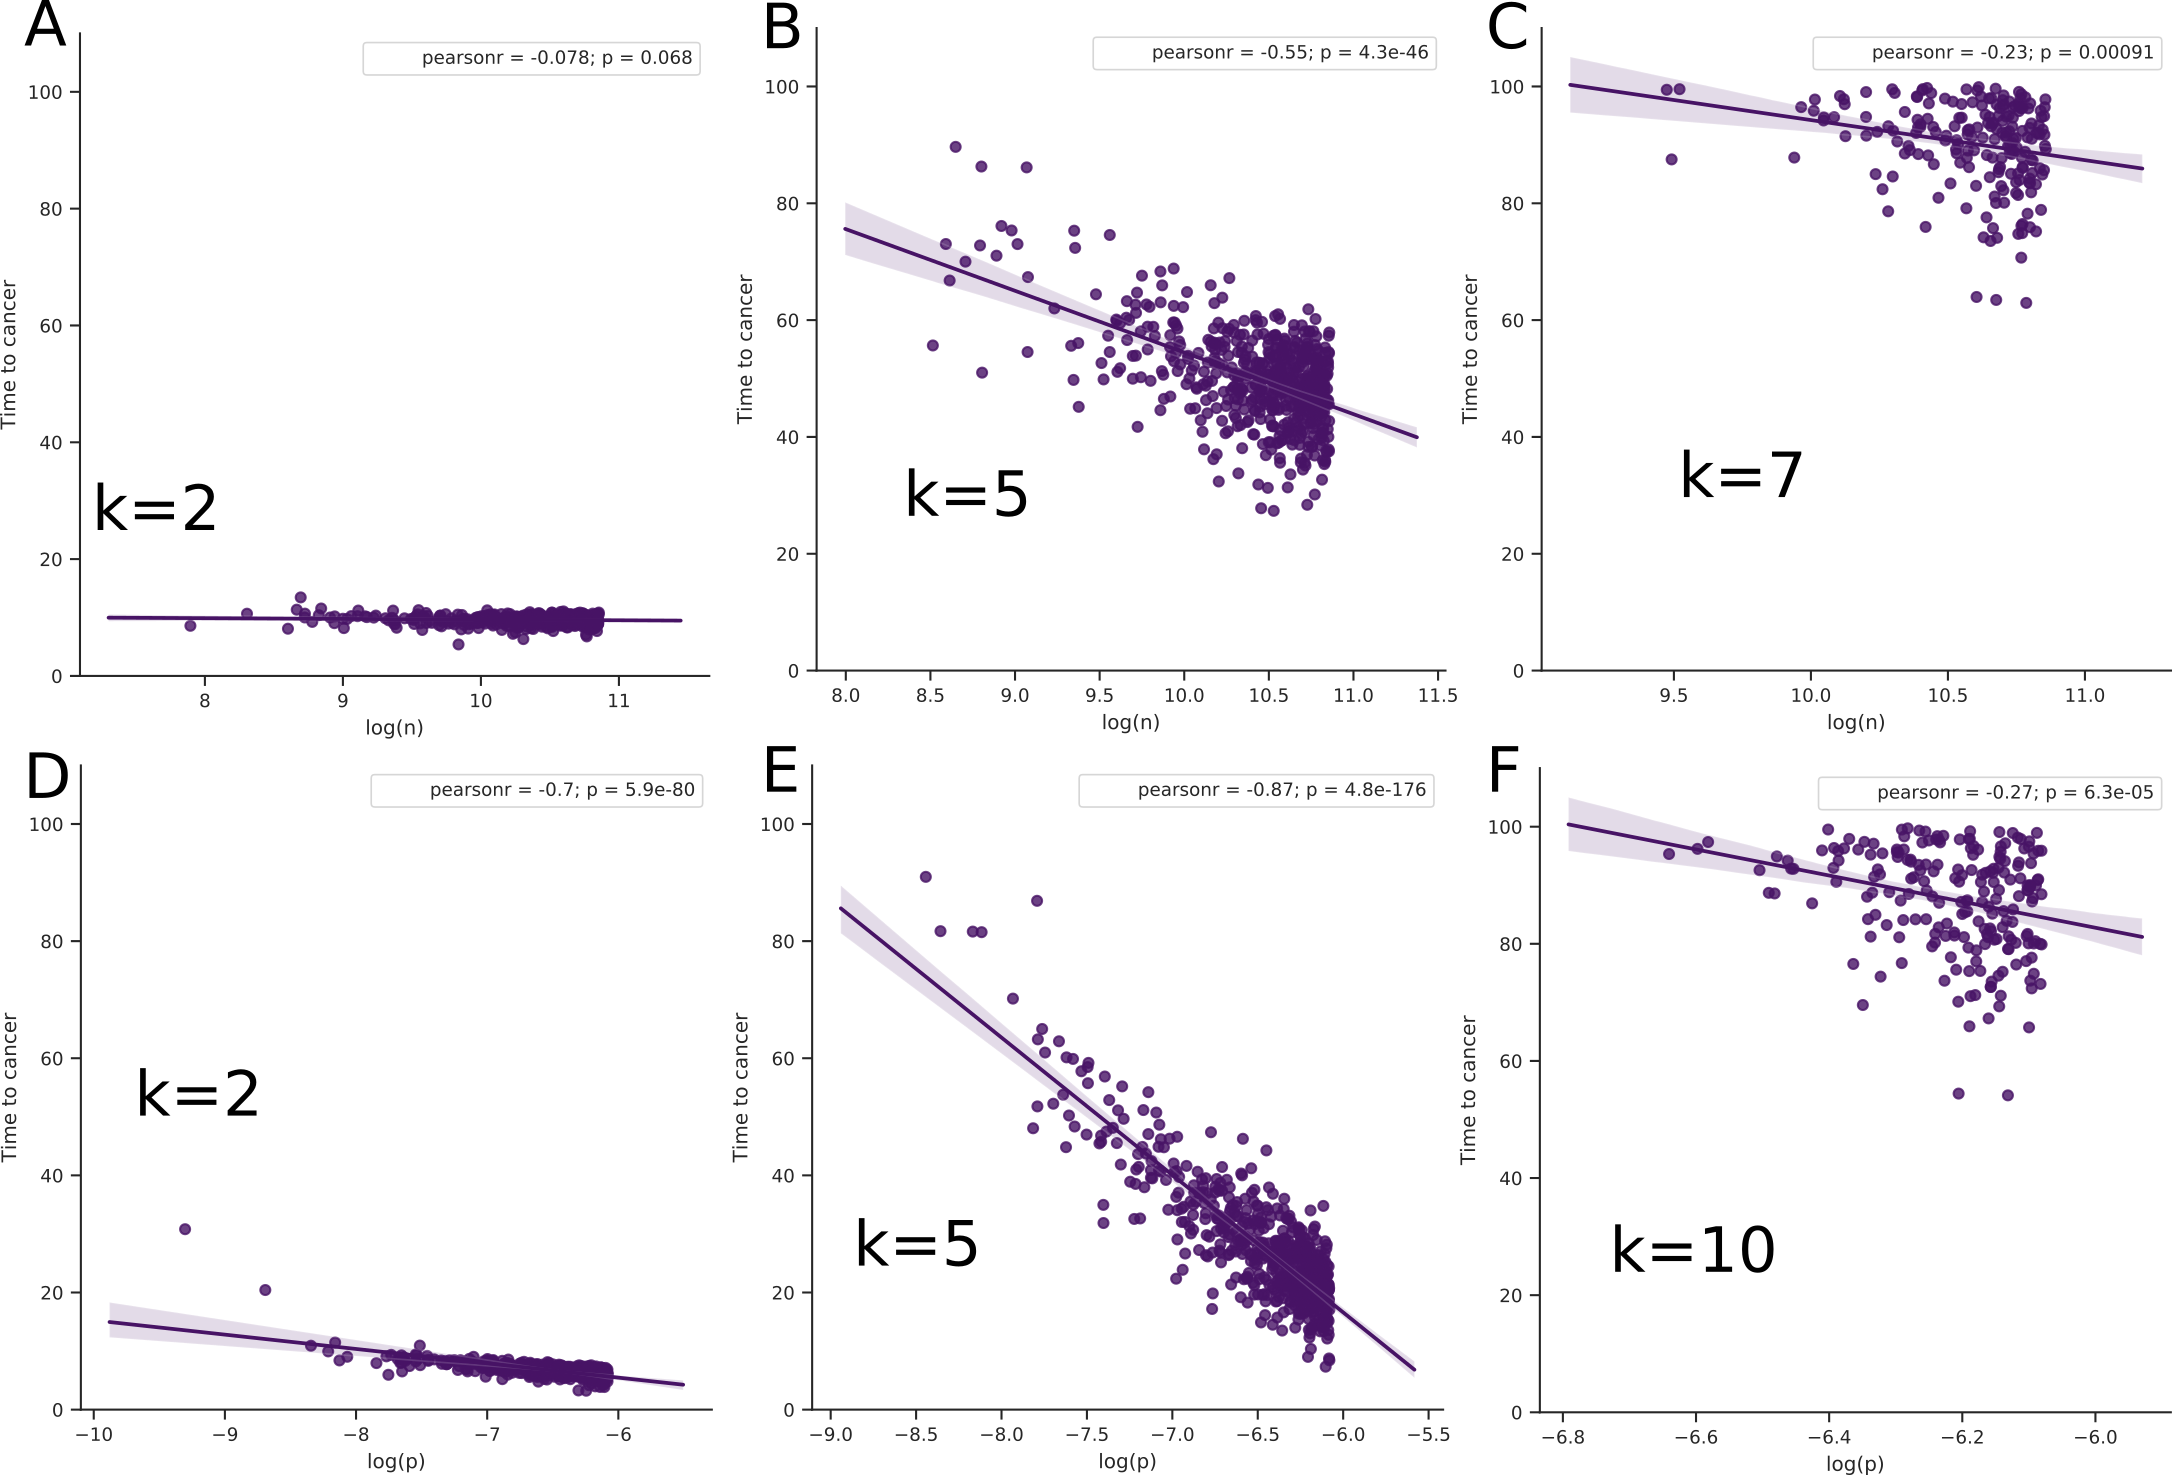
\includegraphics[width=\linewidth, keepaspectratio=true]{figS2-3.png}
			\caption{Effect of $k$ in the context-independent selection case. The plots are time to cancer onset against $log(n)$ or $log(p)$, with $k$ randomized with (A-C) $n$, or (D-F) $p$; value of $k$ in the inset corresponds to the number of threshold oncogenic mutations assumed for the corresponding points. From A to C, for higher threshold of oncogenic mutations, the effect of $n$ on time to cancer gets stronger, as shown by the improvement in the association. For small $k$ however, $n$ does not affect the age of cancer onset. On the other hand, $p$ has a strong effect on the time to cancer at every value of $k$ considered. $k$, $n$ and $p$ were uniformly-distributed random variables with ranges $[0, 20]$, $[1.203*10^{6}, 2.649*10^{10}]$, and $[3.775*10^{-11}, 3.059*10^{-7}]$ respectively. For (A-C), $p=5.603*10^{-9}$. For (D-F), $n=1.785*10^{8}$.}
			\label{figS2.3}
		\end{figure*}

		\begin{figure*}[tbhp]
			\centering
			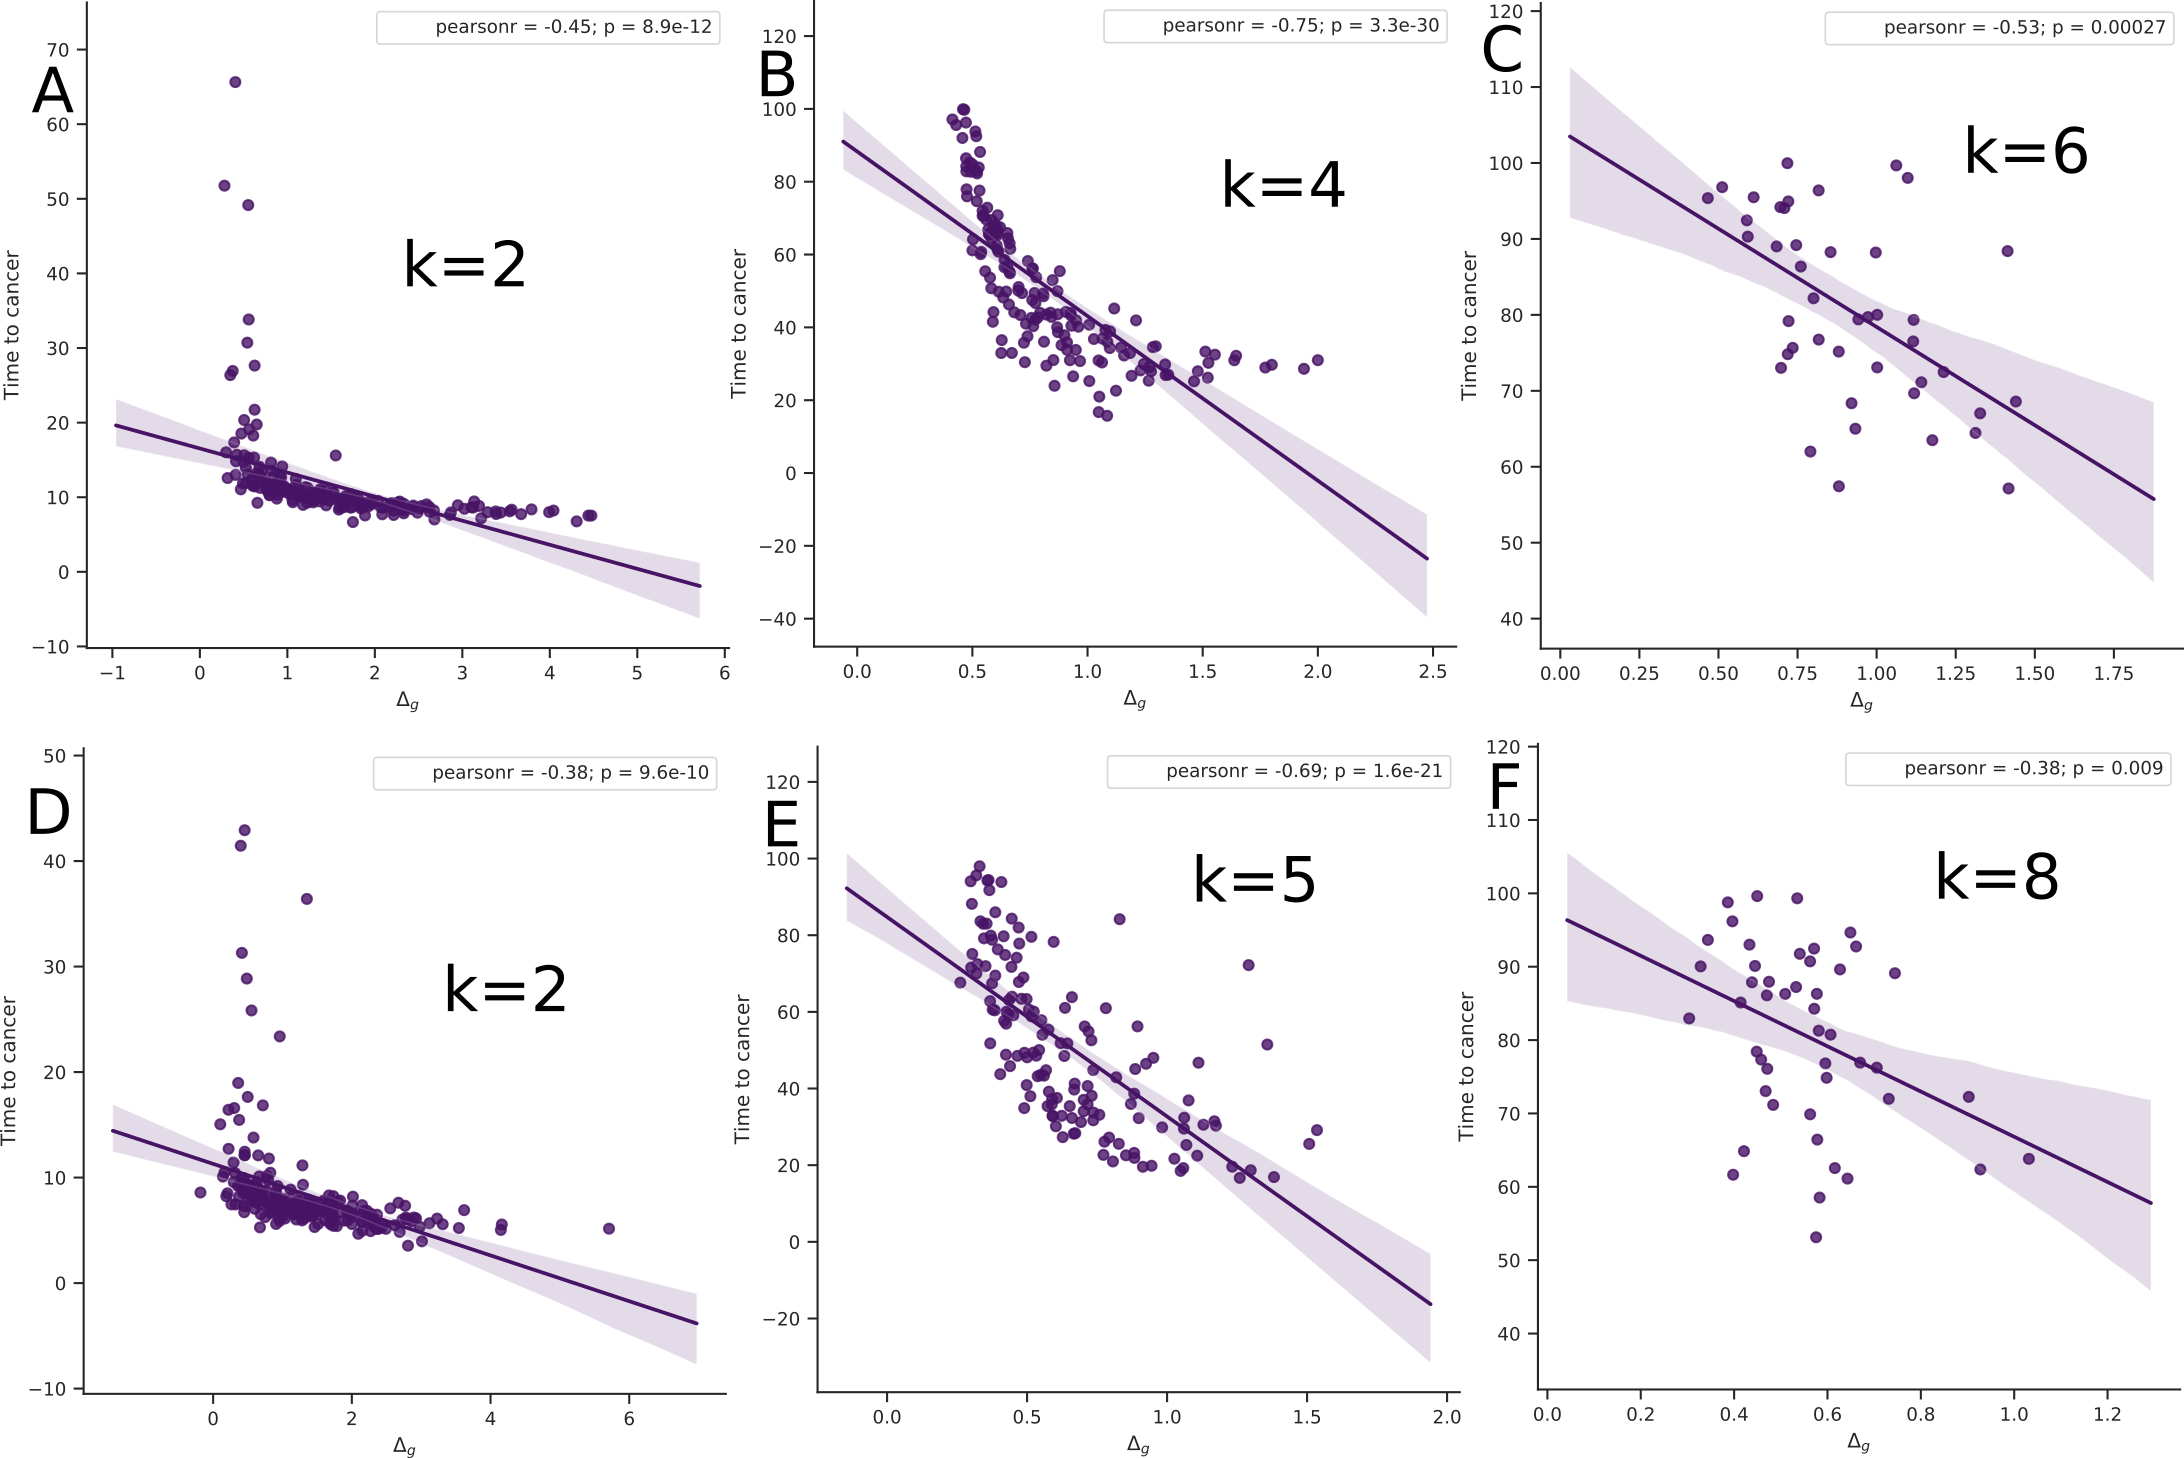
\includegraphics[width=\linewidth, keepaspectratio=true]{figS2-4.png}
			\caption{Effect of $k$ in the context-dependent selection case. The plots are time to cancer onset against $\Delta_{g} = \frac{g_{k}-g_{0}}{k}$ as defined earlier, with $k$ randomized with (A-C) $n$, or (D-F) $p$; value of $k$ in the inset corresponds to the number of threshold oncogenic mutations assumed for the corresponding points. Compared to Figure \ref{figS2.3}, $\Delta_{g}$ explains variance in time to cancer much better than either $n$ or $p$. This is true of both (A-C) when $n$ and $k$ are also randomized, and (D-F) when $p$ and $k$ are also randomized. The effect of $\Delta_{g}$ is nevertheless modulated by the required $k$, as reflected by the range of $\Delta_{g}$ for which cancer occurs; the scale of the x-axis across the figure is indicative of this effect. Ranges of $k$, $n$ and $p$, and the underlying distribution of $g$ are the same as in Figure \ref{figS2.3}. For (A-C), $p=5.603*10^{-9}$. For (D-F), $n=1.785*10^{8}$.}
			\label{figS2.4}
		\end{figure*}

	\begin{refsection}
	\subsection{The nature of the relationship between cancer incidence and cell number}\label{S3 Text}
		\renewcommand{\thefigure}{S3.\arabic{figure}}
		\setcounter{figure}{0}

		\renewcommand{\thetable}{S3.\arabic{table}}
		\setcounter{table}{0}

		\begin{figure}[tbhp]
			\centering
			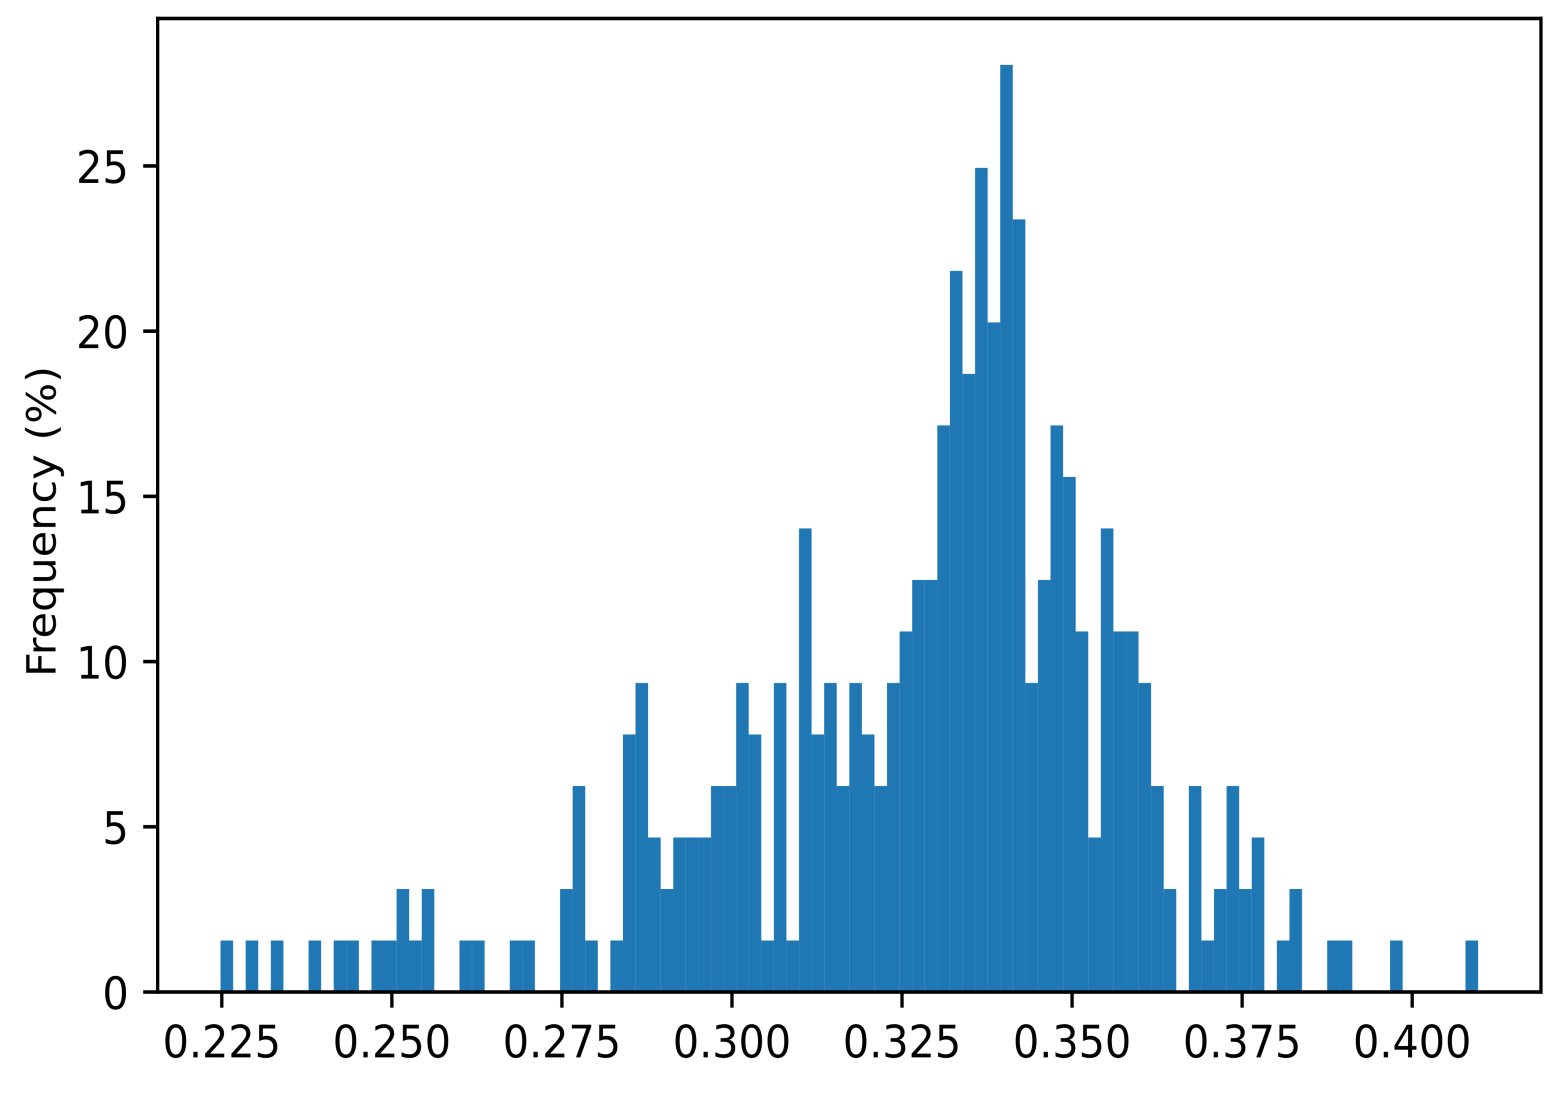
\includegraphics[width=\linewidth, keepaspectratio=true]{lin_slopes.png}
			\caption[Distribution of slopes]{Distribution of slopes of linear regression between \textit{lscd} and cancer incidence on a log-log scale. Of the 423 datasets from corresponding national registries in the IARC database, 347 datasets had values of cumulative incidence rate for all 17 types of cancer considered. All slopes are substantially below unity, indicating non-linear relationships; median slope = 0.334, slope range: 0.225-0.410; median intercept =-13.630, intercept range: (-15.630)-(-11.424)}
			\label{slopes}
		\end{figure}

		\begin{figure}[tbhp]
			\centering
			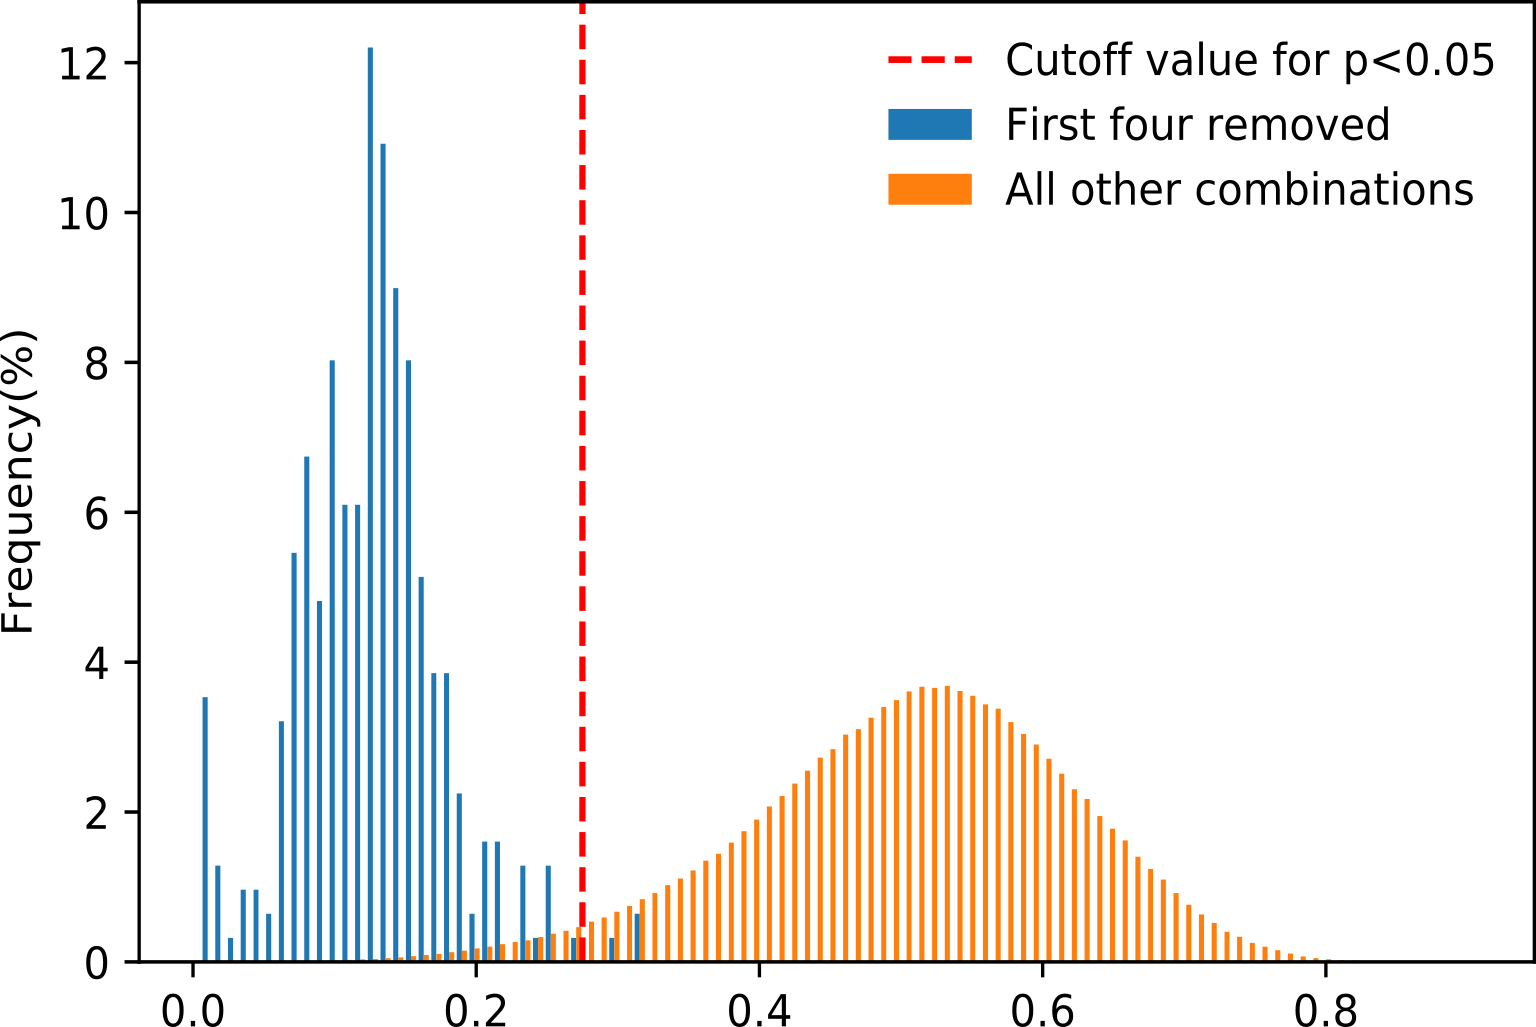
\includegraphics[width=\linewidth, keepaspectratio=true]{elimination.png}
			\caption[Distribution of Pearson's r for reduced datasets]{Distribution of Pearson's r for reduced datasets. The reduced datasets were obtained by removing any four data points from each sample of the IARC dataset, which have 17 data points correponding to the cancer types considered. Linear regression was performed against \textit{lscd} for all possible combinations of removing four points from the sample, resulting in $^{17}$C$_{4}$ = 2380 regression values for every sample, each now with 13 data points. The two distributions correspond to the values of Pearon's r for the combination of the first four points removed, and those for all other combinations pooled respectively. The cutoff refers to the value of r for which p < 0.05, given a sample size of 13 points. The former distribution lies predominantly below this cutoff, suggesting that the linear regression is largely driven only by the first four points. This puts into question the overall inference of linearity.}
			\label{elimination}
		\end{figure}

		\begin{figure*}[tbhp]
			\centering
			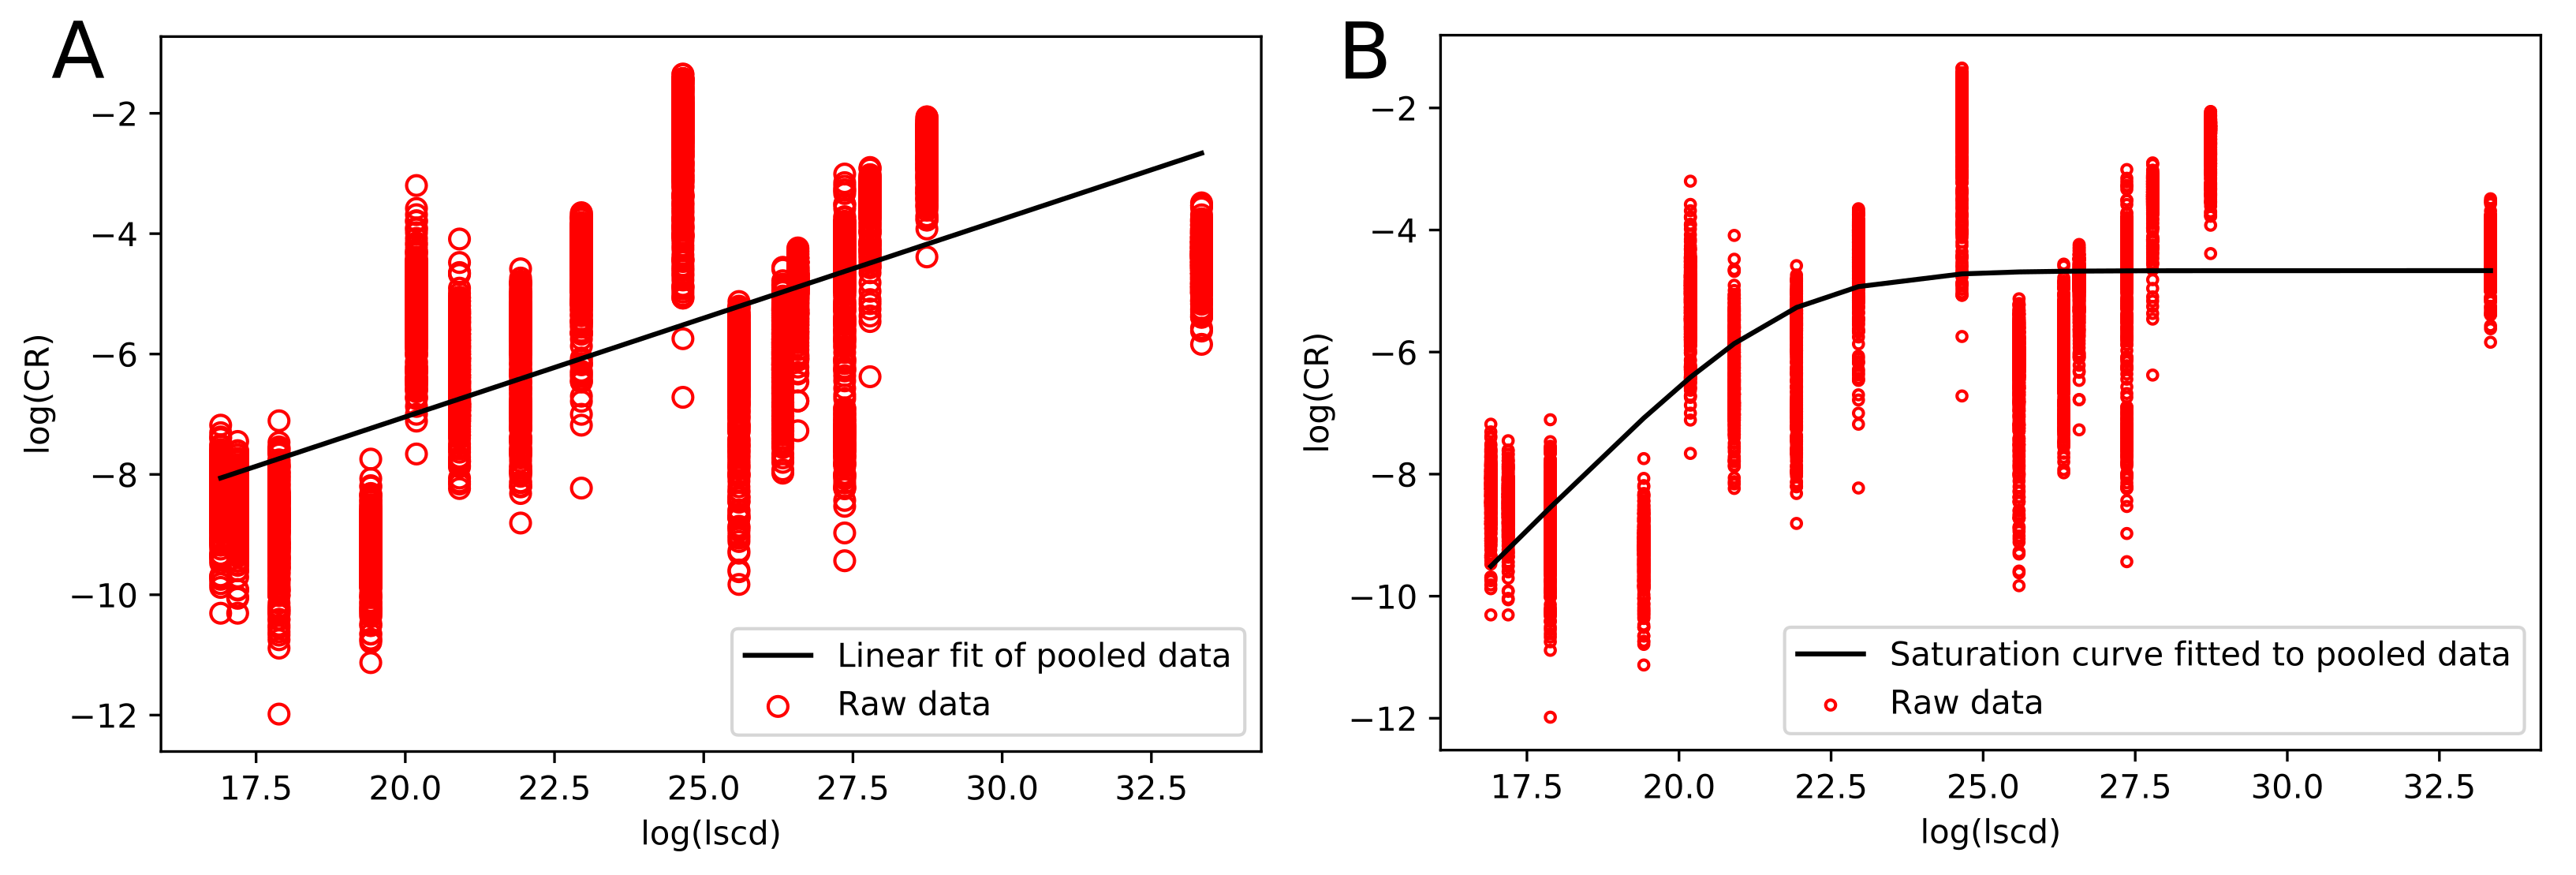
\includegraphics[width=\linewidth, keepaspectratio=true]{figS3-3.png}
			\caption[Distribution of slopes]{A. Linear vs B. Saturation fits. Although for statistical analyses each dataset was used separately, we show pooled data here to facilitate visual impression. Data used are the same as in previous figures.}
			\label{figS3-3}
		\end{figure*}

		\begin{table*}[tbhp]
			\centering
			\begin{tabular}[c]{ccccc}
				\textbf{Regression type} & \textbf{Residuals} & \textbf{First one-fourth} & \textbf{Middle half} & \textbf{Last one-fourth} \\
				\hline
				Linear & Positive & $667$ & $1919$ & $4$ \\
			  	& Negative & $1415$ & $1204$ & $343$ \\
				Saturation & Positive & $1193$ & $1585$ & $220$ \\
			 	& Negative & $889$ & $1538$ & $127$ \\
			 	\hline
			\end{tabular}
			\caption{Number of positive and negative residuals from the linear regression line. The residuals were calculated from linear regressions of cumulative cancer risk, log(CR), against log(\textit{lscd}); data were obtained from IARC as described in the text. The columns correspond to the first one-fourth, middle half and last one-fourth of the \textit{lscd} range. Notably, a substantial skew can be seen in the extremes of the range in the linear case, with more points below the straight line than above it, reflected by a greater number of negative residuals. Compared to the linear case, the skew in the distribution of residuals is significantly lesser for the saturation equation.}
			\label{Table S3.2}
		\end{table*}

		As mentioned in the main text, the last few years have seen two prominent attempts by Tomasetti et al. to examine the relative contributions of spontaneous mutations, genetic and environmental factors in cancer development \cite{Tomasetti78, Tomasetti2017}.  In their analyses, they estimate \textit{l}ifetime \textit{s}tem \textit{c}ell \textit{d}ivisions (\textit{lscd}) for 17 tissue types and correlate them with the incidence of cancer using data from the US, and across the world. In the 2017 paper, they use the IACR datasets for cancer incidence that consisted of 423 databases corresponding to different countries, of which 347 had incidence data for the 17 cancer types considered here. With these data, they report a strong statistical association (Pearson’s r $\approx 0.8$) between \textit{lscd} and incidence of cancer in a given tissue type. The correlations are on a log-log scale, and on that scale, they are considerably strong. At face value, this is in line with the expected relationship if cancer arises out of largely random processes of mutagnesis, and the authors therefore view this association as clear evidence for the causal significance of spontaneous mutations in carcinogenesis. They use this association to further attribute the majority of cancer incidence to random replication errors alone.

		Since all the data used in these papers are publicly available, we performed model fitting exercise, taking a closer look at the nature of the associations. We considered 347 datasets out of the total 423 that had incidence values for all 17 cancer types considered. We find that while Pearson's r was indeed distributed around a median of $0.8$ as reported by Tomasetti et al., but the slopes of the regression were distributed narrowly around a median value of $0.334$ (Figure \ref{slopes}). Going by the classical logic of cancer, it would mean that an average of $0.334$ mutations are required to cause cancer, which is absurd. We expect a positive integer here, but get a substantially small fraction instead. This implies that the hypothesis of $k$ mutations coming together purely by chance is either unsustainable, or has significant gaps that must be addressed.
	
		Residuals from a regression often offer insight on the linearity of a supposed relationship. In this case, we observed that distribution of residuals around the regression was not symmetric, as would be expected based on indication of a strong linear relationship on a log-log scale. Along the first and the last one-fourth of the \textit{lscd} range, the points lie predominantly below the line, while in the middle half of the range, a higher fraction lie above the line, as shown by the respective frequencies of positive and negative residuals (Table \ref{Table S3.2}). In addition to the skewed distribution of points, a visual inspection of Figure \ref{slopes} also suggested that the linear regression itself was largely driven by the first $4$ points in each dataset. In line with this suspicion, upon removal of the first four points, the significance of regression was lost in all $347$ datasets considered in this analysis. In order to test that the loss of significance was not due to reduction in sample size alone, the regression was performed with elimination of all other combinations of four points from each dataset ($^{17}C_{4}-1=2379$ combinations per dataset, not including elimination of the first four). The distribution of Pearson's r values across the combinations revealed a striking difference, with most other combinations of points retaining the significance of the relationship. This is demonstrated by a large part of the former distribution lying below the r value threshold for $p<0.05$ ($r_{threshold}\approx0.55$), as shown in Figure \ref{elimination}. There is therefore evidence to suggest that the linear relationship is largely due to the first four incidences being lower than the rest.
		Taken together, the above analyses point to a significant deviation from a linear relationship on a log-log scale between the cumulative rate and \textit{lscd} suggested by Tomasetti et al. We had observed earlier from linear regression that the slopes had a median of $0.334$. A fractional slope on a log-log scale indicates that on a linear scale, cancer incidence would grow with \textit{lscd} in a curve with gradually decreasing slope.

		\small
		\printbibliography
	\end{refsection}

\end{document}